\chapter{Desarrollo.}
\section{Instalación del servidor PowerTAC y conexión con el broker Sample}

Como parte de la actividad de estudio de la plataforma PowerTAC, fue necesario familiarizarse con el servidor, aprender su configuración básica, y la configuración necesaria para conectarse a uno o varios brokers para hacer que compitan, a su vez, familiarizarse con el ambiente de desarrollo de un broker y su configuración para conectarse a un servidor. A continuación se muestra un resumen de la investigación que se hizo sobre la plataforma.
%no se si sea necesario
\subsection{Power TAC}

Power TAC es una competencia anual que se ha realizado desde 2012, donde se simulan futuros mercados minoristas liberados de energía eléctrica, en la que los competidores son entidades de negocios o ``Brokers'' (En la simulación son agentes Inteligentes) minoristas que compran y venden energía tanto en los mercados al por mayor como al por menor.

Los brokers ofrecen servicios de energía a los clientes a través de contratos tarifarios, y luego deben servir a esos clientes negociando esa energía en el mercado al por mayor. En la competencia los brokers son desafiados a maximizar sus ganancias comprando y vendiendo energía en los mercados mayorista y minorista, sujetos a costos fijos y restricciones, el ganador de un juego o simulación individual es el broker con el saldo bancario más alto al final de la simulación \cite{WKetterJCollinsyMdWeerdtThe2017PowerTAC}.

El mercado minorista está integrado por consumidores y productores pequeños, tales como hogares, pequeñas y medianas empresas, propietarios de vehículos eléctricos, etc. es un mercado de tarifas, en el que los clientes pueden elegir entre ofertas de contratos tarifarios de los brokers competidores, comprando pequeñas cantidades de energía (pequeñas en contraste con el mercado al por mayor).

En el mercado al por mayor los brokers interactúan entre si directamente así como con grandes compañías productoras y otros participantes del mercado al por mayor vendiendo y comprando grandes cantidades de energía, la cual usan para venderla en el mercado al por menor. Los clientes son modelos de usuarios domésticos, empresariales e institucionales de energía eléctrica, así como productores de energía que poseen paneles solares o turbinas eólicas.

\subsection{Servidor}

Debido a que se trata de un proyecto de Maven, lo primero que se hizo fue instalarlo, para esto se descargó de su página oficial el paquete de instalación en un archivo zip: \textsf{http://maven.apache.org/download.cgi}
Para instalarlo, basta con descomprimirlo en la carpeta deseada, en este caso el directorio de instalación elegido fue:\\ \texttt{/usr/local/apache-maven-3.3.9}, 
para usarlo en la terminal, fue necesario agregar la carpeta de instalación: \texttt{/usr/local/apache-maven-3.3.9/bin} 
a la variable de entorno path del sistema.

Para esto se agregó la dirección de la carpeta de instalación a los archivos:\\
\texttt{/etc/environment y /etc/profile}, para resultados inmediatos se usó el comando:\\
\texttt{export PATH=\$PATH:/usr/local/apache-maven-3.3.9/bin}\\

Una vez instalado el software Maven, el siguiente paso fue descargar el archivo zip del proyecto de este enlace:\\ \textsf{https://github.com/powertac/server-distribution/releases/tag/v1.3.2}\\
Al terminar la descarga se descomprimió el archivo zip en la carpeta de trabajo\\
\texttt{/home/Documentos/power tac/} \\
Para ejecutar el servidor nos movemos al directorio raíz del proyecto y escribimos el comando correspondiente al modo que queremos ejecutar, el simulador dispone de tres modos: el modo bootstrap, el modo simulación y el modo web.

\begin{enumerate}
	\item \textbf{Bootstrap:} Es necesario correr este modo previamente a la simulación, en este modo se genera un archivo de datos bootstrap, el cual sirve como datos preliminares para ejecutar el modo simulación, este archivo contiene información del clima, información del mercado de tarifas entre otras cosas.

	\item \textbf{Simulación:} Inicia la simulación de entorno donde varios brokers se conectan al servidor y compiten entre sí.
	\item \textbf{Web: } Despliega un servidor web por el cual se puede arrancar cualquiera de los dos modos del servidor anteriores usando una interfaz gráfica amigable, además en el modo simulación dispone de una herramienta de visualización.
\end{enumerate}

Para correr el simulador en modo bootstrap se usó el siguiente comando:\\
\texttt{mvn -Pcli -Dexec.args=``--boot bootstrap-data ''}\\
Donde \texttt{bootstrap-data} es el nombre que se le pondrá al archive generado.
Para correr el servidor en modo simulación se usó el siguiente comando:\\
\texttt{mvn -Pcli -Dexec.args=``--sim --boot-data bootstrap-data ''}

Una vez más \texttt{bootstrap-data} es el nombre del archivo generado por el modo bootstrap. Hay más parámetros para correr el servidor y estos se toman por default del archivo server.properties el cual contiene la configuración por defecto, algunos de estos parámetros de configuración aparecen en la tabla que aparece en la figura \ref{tab:parametros}.

Por último el comando para desplegar el servidor web es el siguiente:
\texttt{mvn -P web}

Al entrar en la interfaz web del servidor podemos ver que nos muestra un formulario para iniciar cualquiera de los modos anteriores (bootstrap o simulación), este formulario se muestra en la figura \ref{fig:interfazFormularioWeb}.

Para correr el modo simulación desde la interfaz web se pusieron los parámetros de la \ref{tab:parametros}.

\begin{table}[!h]
	\begin{center}
		\begin{tabular}{|p{2.5cm}|p{7cm}|p{4cm}|}\hline
			\textbf{Parámetro} & \textbf{Descripción} & \textbf{Valor} \\ \hline
				Input Bootstrap data:  &El nombre del archivo xml generado en el modo bootstrap. & \texttt{bootstrap-data} \\ \hline
				JMS URL: & La url del JMS del broker, este es el valor default. & \texttt{tcp://localhost:61616} \\\hline
				Brokers  & El nombre de usuario del o los brokers que el servidor esperara a que se conecten. & \texttt{Sample}
			\\ \hline
		\end{tabular}			
	\end{center}
	\caption{ Parámetros del servidor.}
	\label{tab:parametros}
\end{table}

%imagen 

\begin{figure}[!h]
	\centering
	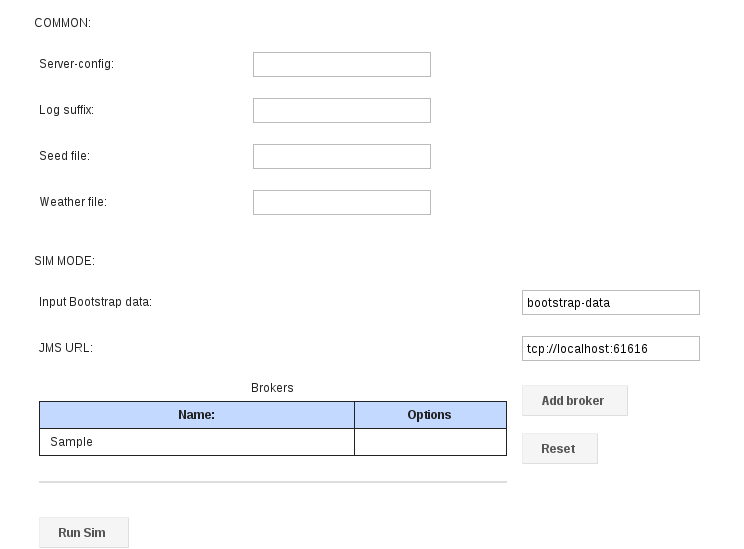
\includegraphics[width=13cm]{img/interfazFormularioWeb.png}
	\caption{Interfaz web del servidor powerTAC}
	\label{fig:interfazFormularioWeb}
\end{figure}

Los otros parámetros (Server-config, Log suffix, Seed file, Weather file) se dejaron en blanco y toman valores por defecto, para propósitos de esta prueba no son necesarios.

Una vez listos los parámetros se inició la sesión dando click en el boton Run Sim, justo abajo del formulario de los parámetros, esto inicia el simulador pero no empieza la simulación %(muestra el mensaje “simulation started”) 
(muestra el mensaje ``simulation started'') 
es decir, no inicio el juego, ya que el servidor quedo en espera del broker Sample.

\subsection{Broker}
Debido a que el broker es en lo que se trabajará agregando funcionalidades, se decidió usar un IDE para tener un buen ambiente de desarrollo, y no solo manejarlo desde la consola como se hizo con el servidor. El IDE elegido para esta prueba fue NetBeans.
Para descargar el broker de ejemplo se usó la herramienta integrada en NetBeans para descargar directamente del repositorio GitHub usando este enlace: \textsf{https://github.com/powertac/sample-broker}\\
En la figura \ref{fig:asistenteNetbeansClonar} se muestra la ventana del asistente de NetBeans para clonar repositorios desde un servidor git.

\begin{figure}[h]
	\centering
	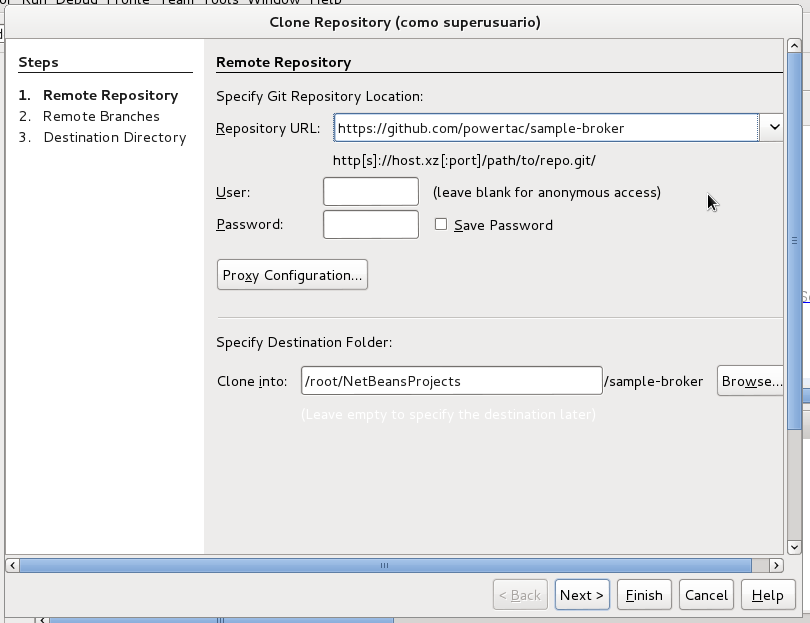
\includegraphics[width=13cm]{img/asistenteNetbeansClonar.png}
	\caption{Asistente de NetBeans para clonar proyectos desde un servidor git.}
	\label{fig:asistenteNetbeansClonar}
\end{figure}

Los parámetros de configuración del broker pueden ponerse en los argumentos a la hora de ejecutarlo desde consola, si estos se omiten, el broker los lee por defecto del archivo broker.properties lo cual resulta útil porque solo hace falta correr el proyecto sin ningún parámetro adicional, haciendo posible ejecutarlo desde NetBeans sin modificar los argumentos de ejecución.

En el archivo broker.properties se encuentran varias propiedades, de ellas son de especial importancia las siguientes:\\

\lstset{language=Xml, label=lst:parametrosBroker, caption={[Archivo \texttt{broker.properties}] Archivo \texttt{broker.properties}},
tabsize=3 ,numbers=left,  stepnumber=1, firstnumber=100}

\begin{lstlisting}[frame=single]  
# - - - - - - - username, password - - - - - - -
samplebroker.core.powerTacBroker.username = Sample
samplebroker.core.powerTacBroker.password = secret
# - - - - - - - - - - - JMS - - - - - - - - - - -
samplebroker.core.jmsManagementService.jmsBrokerUrl =
tcp://localhost:61616
\end{lstlisting}

El valor de la propiedad \texttt{username} de la línea 101 
tiene que coincidir con el parámetro Brokers que se le pasa al servidor al iniciar la simulación, así como también el valor del parámetro \texttt{jmsBrokerUrl} de la línea 104 tiene que coincidir con el parámetro JMS URL de la configuración inicial de la simulación del servidor.\\

Una vez asegurado que los parámetros del broker y el servidor coincidan, se procede a ejecutar el broker, para esto solo damos clic derecho al proyecto y seleccionamos la opción run; 
Si no está seleccionada una clase Main por defecto (que contenga el método main), nos aparecerá una ventana para que seleccionemos la clase a ejecutar, esta es:\\ \texttt{org.powertac.samplebroker.core.BrokerMain}.

Al hacer esto NetBeans se encargara de construir y corre el proyecto usando Maven, al ser NetBeans quien lo ejecuta, no usa ningún parámetro extra en la ejecución por lo que todas las propiedades las lee del archivo \texttt{broker.properties}.

También es posible correr el broker desde la consola del sistema, Para correr el broker desde la consola, es necesario posicionarse en el directorio raiz del proyecto, en este caso es \texttt{/root/NetBeansProjects/sample-broker\#} y simplemente ejecutar el comando:\\
\texttt{mvn compile exec:exec -Dexec.args="--config \\
broker.properties"\\
}

Donde \texttt{broker.properties} es el archivo de configuración que contiene las propiedades del broker (Como el nombre y su JMS URL).
Esto iniciara la descarga de las dependencias necesarias (si aún no se tienen), la construcción del proyecto y la ejecución del broker con los parámetros especificados en el archivo \texttt{broker.properties}, si se desea especificar otro archivo de propiedades es necesario hacerlo en el comando.

\subsection{Servidor en marcha}
La versión web del servidor dispone de una herramienta de visualización web, la cual muestra los resultados de la prueba en tiempo real, después de varios minutos de correr la simulación, la ventana de resultados se parece a la que se muestra en la figura \ref{fig:visualizadorWebResultados}.

\begin{figure}[h]
	\centering
	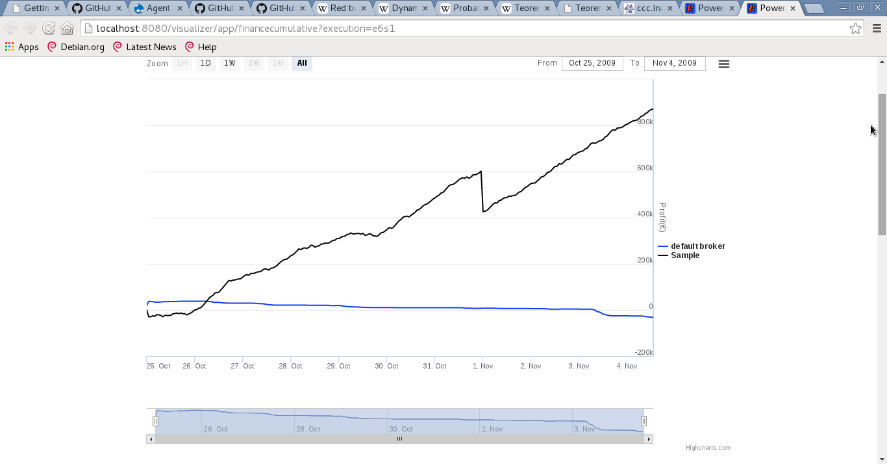
\includegraphics[width=13cm]{img/visualizadorWebResultados.png}
	\caption{Visualizador web de resultados de la simulación.}
	\label{fig:visualizadorWebResultados}
\end{figure}

En la figura \ref{fig:visualizadorWebResultados} el eje $x$ representa el tiempo y el eje $y$ representa la ganancia del broker correspondiente, podemos ver como el Sample broker (el broker que se ejecutó desde NetBeans) inicio con menos ganancias pero conforme
transcurrió el tiempo le gano por mucho al default broker (el broker por defecto que tiene el simulador el cual no ejecuta ninguna estrategia), de igual manera, si hubiera más brokers conectados al servidor estos aparecerían en el gráfico.

Estos resultados de la simulación se guardan además en la carpeta log, que está en la raíz del proyecto, en los archivos \texttt{powertac-sim-0.state} y \texttt{powertac-sim-0.trace}, y cada vez que se corre una simulación el número que en esta primera prueba fue 0, va aumentando.

\section{Estudio de métodos de regresión}
El objetivo es este proyecto es mejorar el broker del INAOE COLDPower, implementando nuevas técnicas que permitan predecir mejor el clima y los patrones de consumo de energía de la población para tomar mejores decisiones y mejorar el rendimiento del broker (aumentar las ganancias en las simulaciones); para llegar a esto fue necesario primero estudiar diversas técnicas de predicción como parte del desarrollo del proyecto, empezando por análisis de regresión. En esta parte del proyecto se llego al siguiente resumen.

Dentro del análisis de regresión hay dos modelos simples por los cuales se
empezó: La regresión lineal y polinomial.

\subsection{Regresión lineal}
El análisis de regresión lineal nos puede ayudar a conocer 3 cosas:

\begin{enumerate}
	\item Si las variables independientes están relacionadas con la variable dependiente, o ayudan a explicar los cambios en la variable dependiente.
	\item Determinar que variables en particular son predictores significativos de la variable dependiente y de qué manera la afectan, la manera en que una variable $x_i$ afecta a la variable dependiente está dada por su coeficiente $\beta_i$ en el modelo generado.
	\item Generar un modelo que muestre como el conjunto de variables predictoras o independientes, pueden ser usadas para predecir valores desconocidos de la variable dependiente y así poder hacer pronósticos. Este modelo naturalmente esta expresado en una ecuación, la cual es una combinación lineal del conjunto de variables independientes.
\end{enumerate}

El estudio de esta técnica fue útil para entender los métodos de regresión en general, ya que es la forma más simple y algunas otras técnicas son parecidas a esta o incluso se basan en ella, como la regresión polinomial, y esta fue el primer tipo de análisis de regresión en estudiarse rigurosamente y en ser usado extensamente en aplicaciones prácticas \cite{XYanLinearRegressionAnalysis}.
Esto es porque los modelos que dependen linealmente de sus variables son más fáciles de ajustar que modelos que son no lineales en cuanto a la relación de sus parámetros y porque las propiedades estadísticas de los estimadores resultantes son más fáciles de determinar.

\subsection{Regresión polinomial}\label{subsec:regresionPolinomial}
Como extensión al algoritmo de regresión lineal, se estudió también el análisis de regresión polinomial y su relación con la regresión lineal, que aunque sirve para describir un modelo donde las variables son no lineales (un polinomio), los parámetros a encontrar son lineales.

Por ejemplo, considere una situación en donde una pequeña pelota se lanza al aire y se miden las alturas $h_i$ mientras haciende, durante varios momentos $t_j$. 
Los valores medidos están en la figura \ref{tab:valoresMedidos}. 
El modelo matemático que describe este fenómeno físico nos dice que, ignorando la resistencia del viento, la relación puede ser modelada como:
$$h_i = \beta_1 t_i + \beta_2 t_i^{2} + \varepsilon_i$$
\begin{table}[!h]
	\begin{center}
		\begin{tabular}{|p{2.5cm}|p{2.5cm}|}\hline
			$t_i$ & $h_1$ \\ \hline
				1 & 2 	\\ \hline
				2 & 6	\\\hline
				3 & 12  \\\hline
				4 & 20  \\\hline
				5 & 30  \\\hline
		\end{tabular}			
	\end{center}
	\caption{Valores medidos.}
	\label{tab:valoresMedidos}
\end{table}


Donde $\beta_1$ determina la velocidad inicial de la pelota, $\beta_2$ es proporcional a la constante de gravitación y $\varepsilon_i$ es debido a los errores de medición y/o a la resistencia del viento.
La regresión lineal puede ser usada para estimar los valores de $\beta_1$ y $\beta_2$  a partir de los datos medidos, aunque los datos solo sean dos variables $h_i$ y $t_i$ , solo que en esta tabla de datos de una variable independiente ($t_i$) se extiende a una tabla de datos con dos variables independientes ($t_i$ y $t_i^{2}$), esta transformación de un modelo de $n$ variables independientes a uno con $n*e$ variables independientes, donde $e$ es el grado del polinomio (el exponente más grande). En este caso $n=1$ ya que disponía de solo una variable independiente, y $e=2$ ya que el grado del polinomio que describe el modelo deseado es cuadrático. Este nuevo modelo se representa en la figura \ref{tab:transformacionModelo}.
% si da tiempo cambiar esto por poner las tablas en dos columnas
\begin{table}[!h]  
	\begin{center}
		\begin{tabular}{|p{2.5cm}|p{2.5cm}|p{2.5cm}|}\hline
				$t_i$ & $t_i^{2}$ & $h_1$  \\ \hline
				1 & 1 & 2 	\\ \hline
				2 & 4 & 6	\\\hline
				3 & 9 & 12  \\\hline
				4 & 16& 20  \\\hline
				5 & 25& 30   \\\hline
		\end{tabular}			
	\end{center}
	\caption{ Transformación del modelo de la tabla de la figura \ref{tab:valoresMedidos}}
	\label{tab:transformacionModelo}
\end{table}

Al aplicar regresión lineal a los datos de la tabla de la figura \ref{tab:transformacionModelo} se obtiene una regresión
polinomial de modelo original representado en la tabla de la figura \ref{tab:valoresMedidos}. 
Este método de transformar el modelo para aplicar una regresión polinomial, se usó en la actividad de Implementación de regresión polinomial en la página \pageref{subsec:implementacionRegresionPolinomial}, a su ves, mas adelante se usa un método parecido a este para hacer análisis de series de tiempo, el cual esta encapsulado en la clase \texttt{WekaForecaster}, parecido en el sentido de que se toma un modelo y se le agregan variables transformándolo en otro modelo que se puede aprender por otro algoritmo de regresión o clasificación cualquiera de la librería weka.

\subsection{Estudio de redes bayesianas} \label{subsec:redesbayesianas}
El estudio de redes bayesianas es necesario ya que se usara este modelo probabilístico como técnica de predicción, más específicamente las redes bayesianas dinámicas, las cuales surgen a partir de las redes bayesianas. Una red bayesiana dinámica o temporal es un modelo estadístico y estocástico que amplía el concepto de red bayesiana.

A diferencia de este último, una red bayesiana dinámica puede representar la evolución de variables aleatorias basándose en una secuencia discreta, por ejemplo, pasos de tiempo. 
El término dinámico caracteriza el sistema modelado, no la red que no cambia.

Como tal lo que se puede calcular con una red bayesiana es la posibilidad de un evento ocurra,
por ejemplo la posibilidad de que una planta eólica produzca entre 40 y 45 kilowatts de energía, o la probabilidad de que el día este soleado, así que no arroja directamente predicciones de variables numéricas (solo de variables nominales), sin embargo se puede calcular el valor esperado a partir de estas probabilidades. Por ello, los campos numéricos son transformados a campos nominales, así que se tienen que discretizar los datos.

Un ejemplo de una red bayesiana sería en el diagnóstico médico, para determinar la probabilidad de un paciente que tiene una enfermedad con base en los síntomas. En la figura \ref{fig:redBayesianaDiagnostico} se muestra un ejemplo de una red bayesiana que modela un diagnóstico médico con base de los síntomas.

\begin{figure}[h]
	\centering
	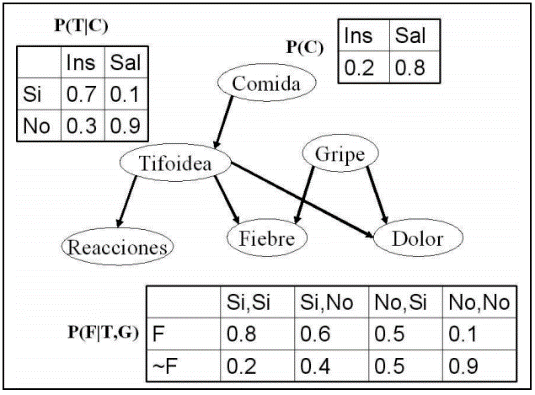
\includegraphics[width=13cm]{img/redBayesianaDiagnostico.png}
	\caption{Red bayesiana que modela un problema de diagnóstico médico.}
	\label{fig:redBayesianaDiagnostico}
\end{figure}

\subsection{Estudio de series de tiempo} \label{subsec:estudiost}
Para comprender el uso de las herramientas para el análisis de series de tiempo primero se hizo una investigación sobre estas de forma general, después una investigación mas enfocada a las herramientas que existen en la librería weka.\\
Una \textit{serie de tiempo} es una secuencia de datos, que representan observaciones o
mediciones de algún fenómeno, indexados por tiempo, mas comúnmente, una
secuencia de observaciones tomadas en puntos sucesivos en el tiempo igualmente
espaciados. Por lo tanto es una secuencia de datos de tiempo discretos. Ejemplos
de una serie de tiempo son la altura de las mareas cada hora, la tasa mensual de
desempleo de los últimos 5 años, el valor de cierre diario de cierta empresa.\\
El \textit{Análisis de series de tiempo} es el proceso de usar técnicas estadísticas para modelar y explicar una serie de puntos (datos) dependientes del tiempo. El \textit{pronóstico de series de tiempo} es el proceso
de  usar un modelo para generar predicciones de futuros eventos basados en los eventos pasados conocidos.
Los datos de series de tiempo tienen un orden temporal natural, esto difiere de aplicaciones típicas de 
machine learning donde cada dato es un ejemplo independiente del concepto que se va a aprender, y el orden
de los datos en el conjunto de dato no importa. 
La librería weka a partir de su version 3.7.3 tiene un ambiente dedicado al análisis de series de tiempo que
permite que modelos de predicción sean desarrollados evaluados y visualizados. Este ambiente viene en un plugin y toma la forma de una pestaña en la interfaz gráfica ``Explorer" de weka y puede ser instalado a través del gestor de paquetes de weka, y para usar la API se puede agregar al proyecto usando Maven agregando al \texttt{POM.xml} en el elemento {\tt \lstinline$ <dependencies>$ } la dependencia que se encuentra en el código \ref{lst:dependency}.
\lstset{language=XML, label=lst:dependency, caption={[Dependencia] Dependencia} } 
\begin{lstlisting}[frame=single]  
<dependency>
	<groupId>pentaho.weka</groupId>
	<artifactId>pdm-timeseriesforecasting-ce</artifactId>
	<version>1.1.1</version>
	<scope>compile</scope>
</dependency>
\end{lstlisting} 
También es necesario agregar el repositorio en donde se encuentra esta dependencia ya que no se encuentra en el repositorio de Maven, para esto hay que agregar las líneas del código \ref{lst:repository} al elemento  {\tt \lstinline$ <repositories>$ }. 

\lstset{language=XML, label=lst:repository, caption={[Repositorio] Repositorio}} 
\begin{lstlisting}[frame=single] 
<repository>
	<id>pentaho-releases</id>
	<url>http://repository.pentaho.org/artifactory/repo/</url>
</repository>
\end{lstlisting}
El framework de weka para las series de tiempo toma un enfoque de machine learning/data mining para modelar series de tiempo transformando los datos en una forma que los algoritmos estándar de aprendizaje proposicional puedan procesar. Esto lo hace quitando el orden temporal de cada fila en el conjunto de datos, y codificando la dependencia del tiempo vía campos adicionales en cada una de las filas. 
Estos campos a veces son llamados variables rezagadas (``lagged variables") o características de interacción (``interaction features"), este proceso es similar a la regresión polinomial discutido en el reporte anterior, ya que este también necesita de dichas variables adicionales. 
Varios otros campos son generados para permitir a los algoritmos modelar tendencias y estacionalidad. 
Después de que los datos han sido transformados, cualquier algoritmo de regresión de weka puede ser aplicado para aprender el modelo, en este periodo se hicieron pruebas con el algoritmo de regresión lineal, pero cualquier método capas de predecir una variable continua puede ser aplicado, incluyendo poderosos métodos no lineales tales como  máquinas de soporte vectorial para regresión (``support vector machines"). Este enfoque de análisis de series de tiempo y pronostico de series de tiempo es a veces mas poderoso y mas flexible que técnicas estadísticas clásicas  tales como ARMA y ARIMA \cite{pentaho}.

\section{Implementación de métodos de regresión usando la librería weka}

Parte de las actividades futuras es crear un software de pronóstico de producción de energía y pronóstico de consumo de energía que después se adaptara al broker para que este pueda tomar mejores decisiones, para esto se implementaran varios algoritmos de regresión y clasificación que están en la librería weka, por lo que el primer paso hacia llegar al este objetivo es aprender a usar la librería weka.

\subsection{Librería weka}
Weka es una colección de algoritmos del área de machine learning, para tareas de minería de datos. Estos algoritmos pueden ya sea aplicarse directamente a un conjunto de datos, o llamarse desde código java mediante la API de weka.
Weka contiene herramientas para el preprocesado de datos, clasificación, regresión, clusterización, reglas de asociación y visualización. También está bien adaptado para el desarrollo de nuevos esquemas de machine learning. 

El nombre proviene de un ave no voladora de naturaleza inquisitiva que vive solamente en la isla de Nueva Zelanda.

Weka es un software de código abierto, bajo la licencia GNU General Public License.

En este periodo se hicieron varias pruebas con la librería weka, empezando por pruebas desde consola, como la de la figura \ref{fig:ejecucionAlgoritmoClasificacion}, con los datos de ejemplo que trae la librería weka, y después se desarrolló un proyecto en java que hace uso de la API de esta librería.

En la figura \ref{fig:ejecucionAlgoritmoClasificacion} se muestra como se ejecutó la clase \texttt{J48} de la librería weka, la cual es una implementación de un algoritmo de clasificación (árbol de decisión). 
El programa recibe el conjunto de datos a clasificar en el archivo \texttt{data/weather.arff}, y recibe como parámetro \texttt{-p} que significa que despliegue los resultados de la clasificación, con los atributos de principio a fin, por eso la especificación ``first-last''.

\begin{figure}[h]
	\centering
	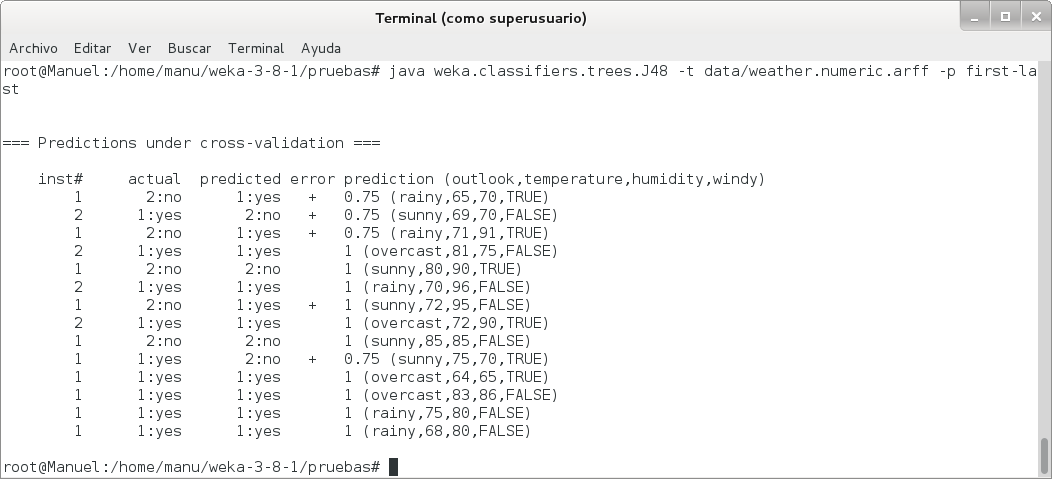
\includegraphics[width=13cm]{img/ejecucionAlgoritmoClasificacion.png}
	\caption{Ejecución de un algoritmo de clasificación de la librería weka.}
	\label{fig:ejecucionAlgoritmoClasificacion}
\end{figure}

\subsection{Extracción de datos} 
\label{subsec:extraccion}
Los datos para hacer las siguientes pruebas fueron recabados usando el broker COLDPower corriendo en el servidor de PowerTAC, este interactúa con el broker enviándole información para que este tome decisiones y responda con diversos tipos de órdenes, tales como ordenes de compra/venta en el mercado al por mayor, creación modificación y eliminación de nuevas tarifas, órdenes de balance, entre otras. La información que el servidor le envía al broker incluye datos sobre el mercado al por mayor y el de tarifas 
(tarifas publicadas por otros brokers), mercado de balance y servicio de contabilidad, el reporte del clima,
información sobre sus clientes (información de producción y consumo de energía entre sus clientes, nuevos subscriptores, clientes que cancelaron subscripción) entre otras, en la figura \ref{fig:activity} se muestra un diagrama de la información compartida entre el broker y el servidor en cada time slot.

La información recogida mediante el broker se guardo en un archivo .arff, que es el formato que usa la librería weka para guardar los \textit{"datasets"} o conjunto de datos; este data set incluye información sobre el clima, y sobre la producción y el consumo de cada tipo de cliente, los archivos generados fueron los siguientes: 

\renewcommand{\labelenumi}{$\bullet$ }
\renewcommand{\labelenumii}{$\bullet$ }
\begin{enumerate}
	\item Consumo:
	\begin{enumerate}
		\item BATTERY\_STORAGE.arff
		\item CONSUMPTION.arff
		\item INTERRUPTIBLE\_CONSUMPTION.arff
		\item ELECTRIC\_VEHICLE.arff
		\item STORAGE.arff
		\item THERMAL\_STORAGE\_CONSUMPTION.arff
	\end{enumerate}
	\item Producción: 
	\begin{enumerate}
		\item FOSSIL\_PRODUCTION.arff
		\item CHP\_PRODUCTION.arff
		\item PRODUCTION.arff
		\item PUMPED\_STORAGE\_PRODUCTION.arff
		\item RUN\_OF\_RIVER\_PRODUCTION.arff
		\item SOLAR\_PRODUCTION.arff
		\item WIND\_PRODUCTION.arff
	\end{enumerate}
\end{enumerate}

Como cada cliente se comporta diferente, se guardaron los kilowatts consumidos o producidos en un archivo por cada tipo de cliente para poder hacer un modelo de predicción para cada uno de ellos que se ajuste a su comportamiento, la figura \ref{fig:datos} muestra el archivo \texttt{SOLAR\_PRODUCTION.arff} 

\begin{figure}[!t]
	\centering
	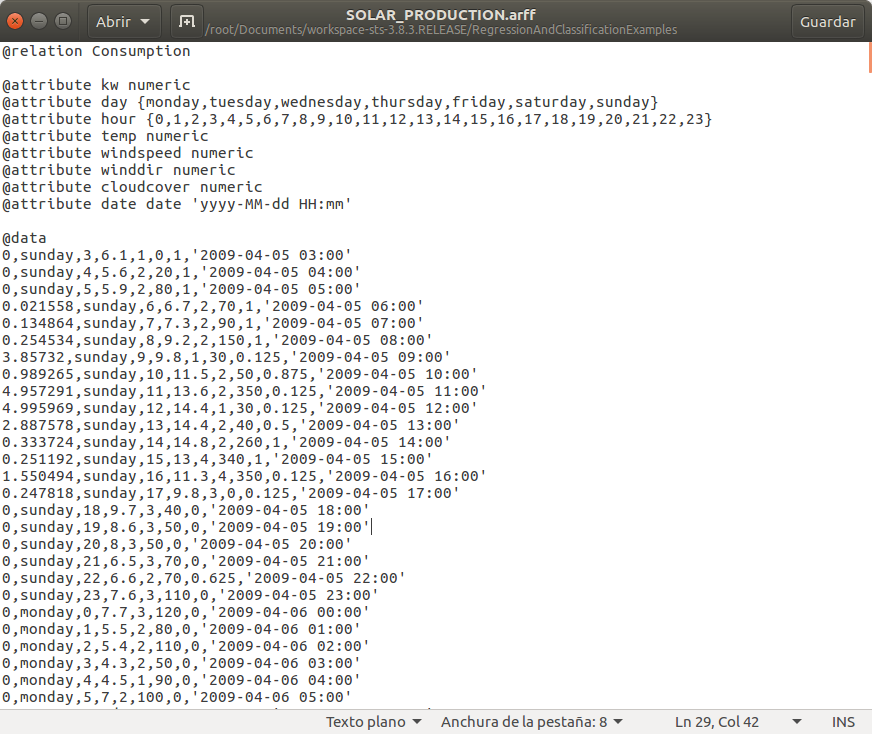
\includegraphics[width=15cm]{img/datos.png}
	\caption{Datos de producción de las plantas solares. }
	\label{fig:datos}
\end{figure}	

En la figura \ref{fig:datos} se pueden ver los campos y sus tipos de datos (numéricos o nominales); el campo \texttt{kw} representa la cantidad total de kilowatts que todas las plantas solares produjeron en el último time slot, esta cantidad es positiva ya que es de producción, para los clientes de consumo esta cantidad es negativa. El campo \texttt{day} representa que día de la semana fue, este es útil para que se tome en cuenta los hábitos de consumo de ciertos tipos de clientes de consumo, como las casas, ya que puede ser que en ciertos días (ejemplo, fines de semana) consuman mas o menos energía. El campo \texttt{hour} tiene el mismo propósito, este también ayuda por ejemplo a predecir la producción de las plantas solares, pues estas tienen un pico de producción al medio día, y disminuye a 0 a medida que se acerca a la noche. El campo \texttt{temp} modela la temperatura, la cual también influye en el consumo de ciertos tipos de cliente, por ejemplo si la temperatura sube los consumidores pueden gastar energía en aire acondicionado, o si baja demasiado pueden empezar a gastar energía en calefacción o almacenamiento térmico (\texttt{thermal storage}). 
Los campos \texttt{windspeed} y \texttt{winddir} modelan la velocidad y dirección del viento, estos datos son cruciales para estimar la producción de las plantas eólicas, así como también el campo \texttt{cloudcover} que modela la nubosidad, es crucial para predecir la producción en las plantas solares. 
Por último el campo \texttt{date} representa la fecha y hora de cuando se tomaron las mediciones, esto es esencial para el modelado de la serie de tiempo, en la librería weka se le conoce también como \texttt{timestamp}.

\subsection{Implementación de regresión lineal}
Después de leer la documentación de la librería weka, se encontraron dos clases que sirven para implementar regresión lineal, la clase \texttt{SimpleLinearRegression}, y la clase \texttt{LinearRegression}; 
ambas hacen regresión lineal, la diferencia es que la clase \texttt{LinearRegression} es una generalización para $n$ variables independientes, y la clase \texttt{SimpleLinearRegression} solo lo hace con una variable independiente con el método de mínimos cuadrados.

Se programó una clase llamada \texttt{LinearRegression} para usar estas clases de dos diferentes maneras, leyendo los datos de un archivo, y generando los datos en tiempo de ejecución. 
En el código \ref{lst:exampleFromFile} se muestra una parte del código usado para correr el algoritmo con los datos que están en el archivo \texttt{lineal.arff} (línea 105).
En la línea 106 se construye el modelo, después inmediatamente se imprime el modelo, vemos en la figura \ref{fig:salidaMetodoLinearRegression} que imprime varias cosas sobre el modelo, y al final imprime la ecuación que describe la recta de mejor ajuste, esta es:
$$class = 1.9988 * a + 0.0158$$
Ya que en el archivo \texttt{lineal.arff} se especificó que la variable dependiente se llama $class$, y la variable independiente se llama $a$, este archivo se construyó con el modelo $class = 2*a + random()*0.5$, por lo cual el modelo generador por el algoritmo es muy parecido.

\lstset{language=Xml, label=lst:exampleFromFile, caption={[Método \texttt{exampleFromFile}] Método \texttt{exampleFromFile}},
tabsize=3 ,numbers=left,  stepnumber=1, firstnumber=100}

\begin{lstlisting}[frame=single]  
public static void exampleFromFile() throws Exception{
	weka.classifiers.functions.LinearRegression classifier= 
		new weka.classifiers.functions.LinearRegression();
	String info=classifier.globalInfo();
	System.out.println(info);
	Instances data=Util.instancesFromFile("lineal.arff");	
	classifier.buildClassifier(data);
	System.out.println(classifier.toString());
	Instance inst= Util.instance(50,100, data);		
	double r=classifier.classifyInstance(inst);
	System.out.println(inst.toString()+": "+ r);		
	Instances curve = data;
	PlotData2D plotdata = new PlotData2D(curve);
	plotdata.setPlotName(curve.relationName());
	plotdata.addInstanceNumberAttribute();
	ThresholdVisualizePanel tvp = new ThresholdVisualizePanel();
	tvp.setROCString("(Area under ROC = " +
		Utils.doubleToString(ThresholdCurve.getROCArea(curve),
		4)+")");
	tvp.setName(curve.relationName());
	tvp.addPlot(plotdata);	
	JFrame jf = new JFrame("Plot for: " + tvp.getName());
	jf.setSize(500,400);
	jf.getContentPane().setLayout(new BorderLayout());
	jf.getContentPane().add(tvp, BorderLayout.CENTER);
	jf.setDefaultCloseOperation(JFrame.DISPOSE_ON_CLOSE);
	jf.setVisible(true);
}
\end{lstlisting}
Las líneas 108 y 109 evalúan un nuevo caso usando el modelo generado, esta instancia tiene los valores de los parámetros $a=50$, $class=100$, y al usar el método \texttt{classifyInstance} en la línea 109, se calcula el valor de la variable $class$ que predice el modelo, en este caso es 99.9581, lo cual se puede ver en la figura \ref{fig:salidaMetodoLinearRegression}, en la línea que dice: 50, 100: 99.958149... la cual corresponde a la impresión de la línea 110 del método \texttt{exampleFromFile()}.
Las líneas siguientes a la 111 son para graficar en una ventana el conjunto de datos usados para crear el modelo, la ventana que creada se puede ver en la figura \ref{fig:representacionGraficaDatosLinearR}.

\subsection{Implementación de regresión polinomial} \label{subsec:implementacionRegresionPolinomial}
Debido a que la librería weka no tiene una implementación directa del algoritmo de regresión polinomial, se hizo uso del método de regresión lineal para poder hacer predicciones de un sistema de naturaleza polinomial. 
Se programó la clase \texttt{PolynomialRegression} que implementa de la interfaz \texttt{weka.classifiers.Classifier}, la cual es la interfaz base para cualquier algoritmo de regresión o clasificación.
Dentro de la clase \texttt{PolynomialRegression} se implementaron los métodos de la interfaz \texttt{Classifier}, los más importantes son los métodos \texttt{buildClassifier} y \texttt{classifyInstance}, que son para construir el modelo a partir de un conjunto de datos y para hacer una predicción dada una instancia respectivamente, 
el método \texttt{buildClassifier} se muestra en el código \ref{lst:PolynomialRegressionBuildClassifier} 
y el método \texttt{classifyInstance} se muestra en el código \ref{lst:PolynomialRegressionChangeInsClassifyIns}.

\begin{figure}[h]
	\centering
	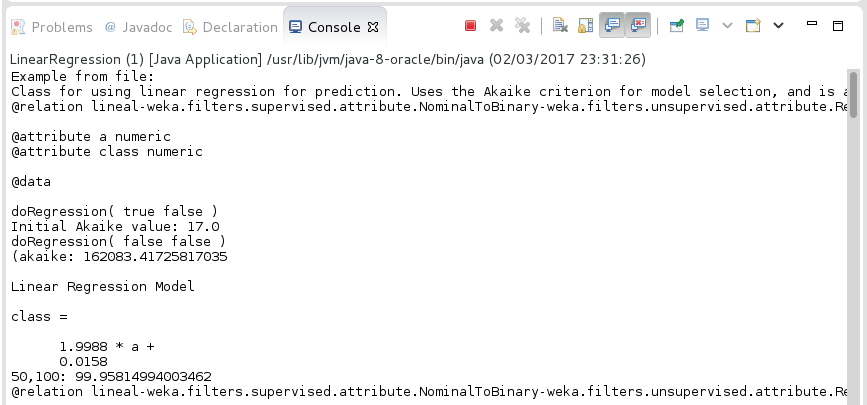
\includegraphics[width=16cm]{img/salidaMetodoLinearRegression.png}
	\caption{Salida del método LinearRegression.exampleFromFile().}
	\label{fig:salidaMetodoLinearRegression}
\end{figure}

\begin{figure}[h]
	\centering
	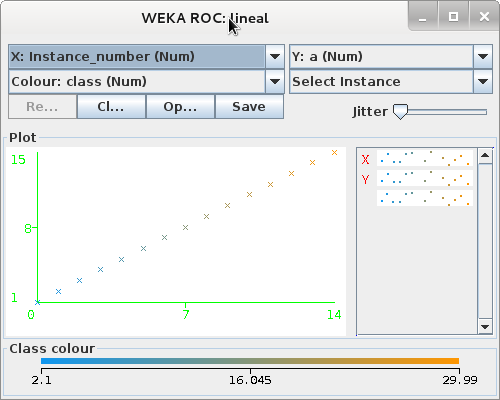
\includegraphics[width=10cm]{img/representacionGraficaDatosLinearR.png}
	\caption{Salida del método LinearRegression.exampleFromFile().}
	\label{fig:representacionGraficaDatosLinearR}
\end{figure}
\clearpage

\lstset{language=Xml, label=lst:PolynomialRegressionBuildClassifier, caption={[Método \texttt{PolynomialRegression.buildClassifier}] Método \texttt{PolynomialRegression.buildClassifier}},
tabsize=3 ,numbers=left,  stepnumber=1, firstnumber=100}

\begin{lstlisting}[frame=single]  
@Override
public void buildClassifier(Instances data) throws Exception {
	if(data.classIndex()<0){
		throw new UnassignedClassException("Class index is "+
			"negative (not set)!");
	}
	ArrayList<Attribute> attribs = new ArrayList<>(
		(data.numAttributes() -1) * degree);
	int att;
	for (att = 0; att < data.numAttributes(); att++) {
		attribs.add(data.attribute(att));
	}
	for (int j = 0; j < data.numAttributes(); j++) {
		if(data.classIndex()==j)
			continue;
		for (int d = 2; d <= degree; d++) {
			StringBuilder sb= new StringBuilder(data.attribute(j)
				.name());
			sb.append("^").append(d);
			attribs.add(new Attribute(sb.toString()));
		}
	}
	Instances newInstances = new Instances(data.relationName()+
		"polynomial", attribs, data.numInstances());
	for (int in = 0; in < data.numInstances(); in++) {
		Instance inst= data.get(in);
		Instance newInst = changeInstance(inst, 
			newInstances.numAttributes());
		newInstances.add(newInst);
	}
	instances= newInstances;
	instances.setClassIndex(data.classIndex());
	classifier.buildClassifier(newInstances);
}
\end{lstlisting}

Como se está usando el método de regresión lineal para hacer regresión polinomial, primero se tiene que hacer una transformación del modelo, la cual se explica en el apartado Regresión polinomial, en la página \pageref{subsec:regresionPolinomial},
esta transformación del modelo se lleva a cabo en el código \ref{lst:PolynomialRegressionBuildClassifier} desde la línea 106 hasta la línea 131, dejando solamente a la línea 132, la cual es la que se encarga de mandar a llamar el método de regresión lineal sobre la nueva instancia del modelo.

El método \texttt{buildClassifier} hace uso del método \texttt{changeInstance}, el cual es una implementación de la transformación del modelo explicado en la sección Regresión polinomial, 
este convierte una sola fila de la tabla de la figura \ref{tab:valoresMedidos} (pagina \pageref{tab:valoresMedidos}) en una sola fila de la tabla de la figura \ref{tab:transformacionModelo} (pagina \pageref{tab:transformacionModelo}), agregándole los parámetros que necesarios para hacer la regresión polinomial. 
El método \texttt{changeInstance} se muestra en el código \ref{lst:PolynomialRegressionChangeInsClassifyIns}, donde también se muestra la implementación del método \texttt{classifyInstance}, el cual también hace uso del método \texttt{changeInstance}, para convertir instancia (única medición de las variables independientes) en una instancia a la cual se le puede aplicar la regresión.
%aqui podria ir una explicacion al metodo changeInstance
En la linea 101 del código \ref{lst:PolynomialRegressionChangeInsClassifyIns} se crea el arreglo que representara a la instancia transformada (una fila de la tabla), el for de la linea 103 llena los primeros elementos con los de la instancia original, el for de la linea 106 llena los demás elementos con 
variables que representan potencias de las variables originales (excepto por la variable de clase por eso el if de la linea 107), de acuerdo con el grado elegido (atributo \texttt{degree}), de tal manera que si la instancia consta de las variables $\{x1,x2,y\}$ donde y es la variable de clase, y el grado es 3, la instancia resultante tendrá las variables $\{x1,x2,y,x1^2,x1^3,x2^2,x2^3\}$ 

La clase \texttt{PolynomialRegression} se prueba desde el \texttt{main} de la clase principal del proyecto el cual se muestra en el código \ref{lst:mainPolynomialRegression}, en este se construye un conjunto de datos modelados por la ecuación $y= x^{2}$ (lineas 102-107), luego se construye el modelo en la línea 108 y de las líneas 109 a la 112 se hace un pronóstico para una instancia en la cual la variable independiente es igual a 20, y según el modelo que se usó para construir los datos, la variable independiente debería de ser $20^{2}= 400$.
El resultado de correr este código fue 399.9999997, una aproximación bastante cercana, con un error casi despreciable, lo cual demuestra que la implementación del algoritmo es buena.

\lstset{language=Xml, label=lst:PolynomialRegressionChangeInsClassifyIns, 
caption={[Métodos \texttt{changeInstance} y \texttt{classifyInstance} de la clase \texttt{PolynomialRegression}] 
Métodos \texttt{changeInstance} y \texttt{classifyInstance} de la clase \texttt{PolynomialRegression}},
tabsize=3 ,numbers=left,  stepnumber=1, firstnumber=100}

\begin{lstlisting}[frame=single]  
protected Instance changeInstance(Instance inst, int numAtt){
	double values[]=new double[numAtt];
	int att;
	for (att = 0; att < inst.numAttributes(); att++) {
		values[att]=inst.value(att);
	}
	for(int j=0;j<inst.numAttributes();j++){
		if(inst.classIndex() == j){
			continue;
		}
		double aux= values[j];
		for (int d= 2; d <= degree; d++) {
			aux*=values[j];
			values[att++]= aux;
		}
	}
	Instance newInst = new DenseInstance(1.0, values);
	return newInst;
}
@Override
public double classifyInstance(Instance instance) 
		throws Exception {
	instance.setDataset(instances);
	Instance newInst= changeInstance(instance,
		instances.numAttributes());
	classifier.setEliminateColinearAttributes(false);
	return classifier.classifyInstance(newInst);
}
\end{lstlisting}




\lstset{language=Xml, label=lst:mainPolynomialRegression, 
caption={[Main para probar la clase PolynomialRegression \texttt{PolynomialRegression}] 
Main para probar la clase PolynomialRegression \texttt{PolynomialRegression}},
tabsize=3 ,numbers=left,  stepnumber=1, firstnumber=100}

\begin{lstlisting}[frame=single]  
public static void main(String[] ar){
	PolynomialRegression classifier= new PolynomialRegression(3);
   	double datos[][]=new double[100][2];
  	for (int i = 0; i < datos.length; i++) {
		datos[i][0]= i;
		datos[i][1]= i*i;
	}
   	Instances ins= instancesFromArrays(datos);
   	classifier.buildClassifier(ins);
   	double x[]=new double[2]{20,400};
   	double y=classifier.classifyInstance(
   		new DenseInstance(1.0,x));
   	System.out.println("y= "+y);   	
}
\end{lstlisting}

\subsection{Implementación de algoritmo de series de tiempo} \label{subsec:implementacionSeries}

La librería weka dispone de una implementación de un algoritmo para analizar series de tiempo el cual toma como base otro algoritmo de la librería que pueda manejar datos numéricos, tal como se vio en la sección \ref{subsec:estudiost} en la \hyperref[subsec:estudiost]{página \pageref{subsec:estudiost}}, este módulo también dispone de una clase para graficar las series de tiempo el cual se uso para ayudar a analizar los resultados de manera mas intuitiva.\\
En la \hyperref[fig:diagramaUml]{figura \ref{fig:diagramaUml}} 
se muestra un diagrama con la implementación del algoritmo de series de tiempo en la clase \texttt{TimeSeries}, el cual hereda de la clase \texttt{AbstractClassifier} para heredar los métodos base de cualquier algoritmo de regresión o clasificación de la librería, y poder usarla junto con otras clases de la librería. La clase implementa de \texttt{TSForecaster} ya que esta interfaz es la que define un analizador de series de tiempo, y esto permite que se use con otras clases de la librería como \texttt{JFreeChartDriver} que sirve para graficar los resultados del análisis, o \texttt{TSEvaluation} que sirve para evaluar el modelo generado.
\begin{figure}[!b]%Ambiente ’figure’
	\centering
	%imagen sin escalar
	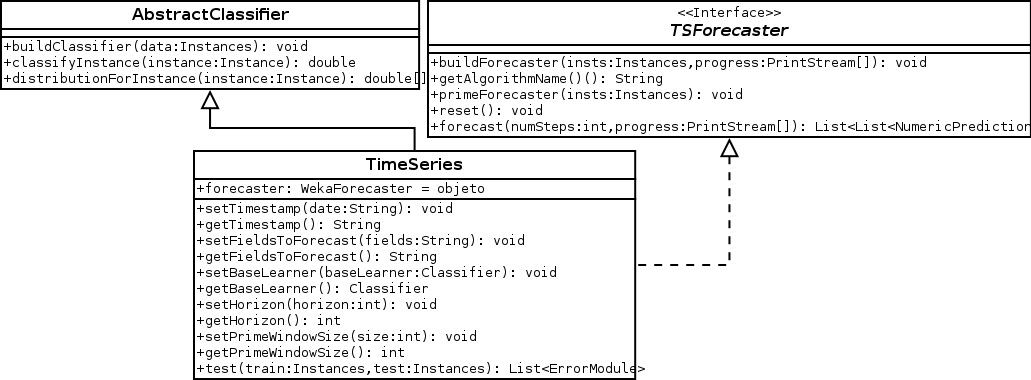
\includegraphics[width=15cm]{img/diagramaUml.png}
	\caption{Diagrama UML de las clases implicadas a la clase \texttt{TimeSeries}. }
	\label{fig:diagramaUml}
\end{figure}

El objeto \textit{forecaster} de la clase \texttt{WekaForecaster} es el motor de esta clase, implementa el algoritmo de pronóstico de series de tiempo. Hace uso de la clase \texttt{TSLagMaker} que es la que crea todas las variables rezagadas o lagged variables, la creación de atributos o campos periódicos, etc.
Los métodos heredados de la clase \texttt{AbstractClassifier} son:
%\renewcommand{\labelenumi}{$\bullet$ }
%\renewcommand{\labelenumii}{$\bullet$ }
\begin{enumerate}
	\item \texttt{buildClassifier(Instances data)} es el método que realiza el análisis de la serie de tiempo y construye el modelo 		a partir de los datos contenidos en el objeto data de la clase \texttt{Instances} que se le paso como parámetro.
	
	\item \texttt{classifyInstance(Instance instance)} es el método que realiza la predicción, recibe un objeto \texttt{Instance}, del cual 	extrae la fecha y retorna una predicción de la variable objetivo para esa fecha.
	
	\item  \texttt{distributionForInstance(Instance instance)} se usa cuando el algoritmo de clasificación/regresión tiene una 				variable objetivo (el atributo cuyo valor intenta calcular) de tipo nominal (discreto) como es el caso de la red bayesiana, que 		retorna un valor de probabilidad para cada uno de los posibles valores de la variable, así que en este algoritmo no se usa.
\end{enumerate}
Los métodos implementados de la interfaz \texttt{TSForecaster} son los que le dan la funcionalidad para el análisis y pronostico de series de tiempo a la clase, \textit{``TSForcaster"} es abreviación de \textit{time series forecaster} o \textit{pronosticador de series de tiempo}. Los métodos de esta interfaz son: 
\begin{enumerate}
	\item \texttt{buildForecaster(Instances insts, PrintStream... progress)} analiza el conjunto de datos en el objeto
			\texttt{insts} y crea el modelo que describe la serie de tiempo. El parámetro \texttt{progress} es un arreglo de flujos 
			donde se imprimirán mensajes de depuración acerca de la ejecución del método, un ejemplo es pasar como parámetro
			\texttt{System.out}.
			
	\item \texttt{getAlgorithmName()} retorna el nombre de la clase que se esta usando para aprender el modelo, en el caso del
			código \ref{lst:tsevaluation}, este método imprimiría: \\ \texttt{weka.classifiers.functions.LinearRegression}.
			
	\item \texttt{primeForecaster(Instances insts)} prepara el modelo (potencialmente) entrenado con datos conocidos hasta el punto 
			actual, para que a partir de ese punto se hagan predicciones hacia el futuro. Se puede usar el mismo conjunto de datos
			usado en el entrenamiento. 
			
	\item \texttt{reset()} reinicia el modelo.
	
	\item \texttt{forecast(int numSteps, PrintStream... progress)} retorna una lista de \texttt{numSteps} listas, donde cada una
			representa las predicciones de la(s) variable(s) objetivo hasta \texttt{numSteps} unidades de tiempo hacia el futuro,
			información del avance del	proceso se imprime en los objetos \texttt{progress}.
\end{enumerate}

La clase (\texttt{TSEvaluation}) automatiza la evaluación del modelo generado, en el código \ref{lst:tsevaluation} se muestra un ejemplo de su uso. 

\lstset{language=Java, label=lst:tsevaluation, caption={[TSEvaluation] Evaluación con la clase \texttt{TSEvaluation}},
tabsize=3 ,numbers=left,  stepnumber=1, firstnumber=100}

\begin{lstlisting}[frame=single]  
Instances datos = Util.instancesFromFile("SOLAR_PRODUCTION.arff");
TimeSeries timeseries = new TimeSeries();
timeseries.setTimestamp("date");
timeseries.setFieldsToForecast("kw");
timeseries.setBaseLearner(new LinearRegression());
int numInstPred=24, size=datos.numInstances();
Instances train = new Instances(datos, 0, size - numInstPred);
Instances test = new Instances(datos,size-numInstPred,numInstPred);
try {
	TSEvaluation evaluation= new TSEvaluation(train, test);		
	PrintStream prog[]=new PrintStream[0];
	evaluation.setHorizon(24);
	evaluation.setPrimeWindowSize(24);
	evaluation.evaluateForecaster(timeseries, true,prog);
	System.out.println(
		evaluation.printPredictionsForTestData("Resultados","kw",1));
	System.out.println(evaluation.toSummaryString());
} catch (Exception e) {
	e.printStackTrace();
}
\end{lstlisting}
En la línea 100 se cargan los datos del archivo \texttt{SOLAR\_PRODUCTION.arff}, de la línea 101 a la 104 se crea y configura el objeto de la clase \texttt{TimeSeries} que realizara el análisis y construcción del modelo, a este se le tiene que decir que campo es el que representa la dimension del tiempo en la serie (línea 102), también se tiene que especificar cuales son los campos objetivos (los que se quieren predecir), en este caso se eligió los kilowatts producidos por la planta solar (línea 103), y lo mas importante se tiene que especificar el algoritmo de aprendizaje a usar, para esta prueba se eligió la regresión líneal (línea 104).
De la línea 105 a la 107 se separan los datos del archivo \texttt{SOLAR\_PRODUCTION.arff} en dos partes, la mayoría se pone en el objeto \texttt{train} que es el que se usara para construir el modelo, este contiene todos excepto los últimos 24 registros, estos últimos registros se ponen en el archivo \texttt{test}, que sera usado para probar el modelo generado y medir su precision.
En la línea 109 se crea el objeto \texttt{evaluation} de la clase \texttt{TSEvaluation} pasandole los datos de entrenamiento y pruebas. Como no se desea imprimir el progreso se crea el arreglo \texttt{prog} de tamaño 0 en la línea 110 y  antes de ejecutar la evaluación se ejecutan las líneas 111 y 112 que especifican el numero de unidades de tiempo a predecir.
\\Por ultimo se ejecuta el método \texttt{evaluateForcaster()} que recibe el objeto que contiene el modelo de la serie de tiempo (este debe implementar la interfaz \texttt{TSForecaster}), un booleano que significa que debe construir el modelo, y el arreglo de flujos donde se imprimirá el progreso. 
Lo que hace la clase \texttt{TSEvaluation} es evaluar hacer varias predicciones un paso adelante, luego predicciones 2 pasos adelante, hasta llegar a predicciones $n$ pasos hacia el futuro, en este caso $n=24$.
Los resultados se imprimen en las líneas 104 y 106, la primera imprime los valores predichos $n$ pasos hacia adelante por el modelo, su valor real y el error que hubo, la segunda línea imprime un resumen de los resultados, que consta de el valor del error medio absoluto y la raíz del error cuadrático medio de cada conjunto de predicciones a $n$ pasos. En la  \hyperref[fig:resultadosEvaluacion]{figura \ref{fig:resultadosEvaluacion}} se muestra la salida de este código. 

\begin{figure}[!h]
	\centering
	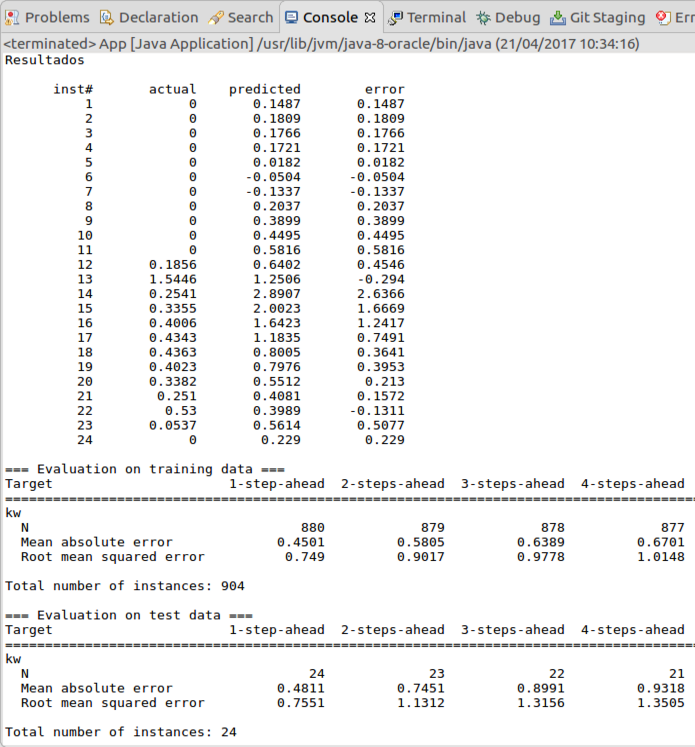
\includegraphics[width=15cm]{img/resultadosEvaluacion.png}
	\caption{Resultados de la evaluación con la clase TSEvaluation. }
	\label{fig:resultadosEvaluacion}
\end{figure}
%\clearpage
La clase \texttt{TSEvaluation} resulta útil para medir la exactitud que tienen las predicciones de acuerdo a cuantos pasos en el futuro se esta prediciendo, no obstante necesitamos una medida de la exactitud para una sola predicción de $n$ pasos hacia el futuro, en lugar de mediciones agrupadas por pasos, es decir $n$ predicciones de 1 paso, $n-1$ predicciones de 2 pasos, $n-2$ predicciones de 3 pasos, tal como lo hace esta clase, por lo que se opto por crear métodos propios para evaluar la exactitud de los resultados, y métodos para graficar los resultados.
El \hyperref[lst:maincustomtest]{código \ref{lst:maincustomtest}} realiza una evaluación de las predicciones a 24 horas generadas por el modelo, y despliega el error medio absoluto junto con otras métricas de evaluación de la exactitud del modelo generado, ademas de mostrar una ventana con un gráfico representando la serie de tiempo real, y la parte generada por el modelo.

\lstset{language=Java, label=lst:maincustomtest, caption={[Evaluación personalizada de series de tiempo] Evaluación personalizada de series de tiempo},
tabsize=3 ,numbers=left,  stepnumber=1, firstnumber=100}

\begin{lstlisting}[frame=single]  
Instances datos = Util.instancesFromFile("SOLAR_PRODUCTION.arff");
String targetName="kw" ;
String xaxis="date";

TimeSeries timeseries = new TimeSeries();
timeseries.setDebug(true);
timeseries.setTimestamp(xaxis);
timeseries.setFieldsToForecast(targetName);
timeseries.setBaseLearner(new LinearRegression());

String period="day=>=*:*:*:*:*:*:*:6:*:* <=*:*:*:*:*:*:*:18:*:*";
timeseries.forecaster.setTSLagMaker(new NewLagMaker());
NewLagMaker lag=(NewLagMaker)timeseries.forecaster.getTSLagMaker();
lag.setIncludePowersOfTime(false);
lag.setIncludeTimeLagProducts(false);
lag.setPrimaryPeriodicFieldName("hour"); 
lag.addCustomPeriodic(period);

int numInstPred=24;
int size=datos.numInstances();
Instances train = new Instances(datos, 0, size - numInstPred);
Instances test = new Instances(datos,size-numInstPred,numInstPred);
timeseries.setHorizon(24);
timeseries.setPrimeWindowSize(24);
List<ErrorModule> preds= timeseries.test(train, test);
JFreeChartDriver chart = new JFreeChartDriver();
List<Integer> stepsToPlot= new ArrayList<>(2);
stepsToPlot.add(1);
JPanel graph;
//graph= Util.graphSeries(preds.get(0), datos, targetName, xaxis);
graph= chart.getGraphPanelSteps(timeseries, preds, targetName,
	stepsToPlot, 0, train);
JFrame jf = new JFrame("Time series");
jf.setDefaultCloseOperation(JFrame.DISPOSE_ON_CLOSE);
jf.setSize(800, 600);
jf.getContentPane().setLayout(new BorderLayout());
jf.getContentPane().add(graph, BorderLayout.CENTER);
jf.setVisible(true);
System.out.println("Mean absolute error: " +timeseries.getMAE());
System.out.println("Mean squared error: "+ timeseries.getMSE());
System.out.println("Root mean squared error: "
	+ timeseries.getRMSE());
System.out.println("Mean absolute percentage error: " 
	+ timeseries.getMAPE());
\end{lstlisting}

En el \hyperref[lst:maincustomtest]{código \ref{lst:maincustomtest}}, de las líneas 100 a la 102 esta especificada la configuración general, la cual es el nombre del archivo donde sacar los datos, el nombre de la variable objetivo o campo a pronosticar, y el campo de fecha que le daré la característica de serie de tiempo a los datos. Es necesario especificar porque puede ser que tenga mas de un campo de fecha y solo uno representa el eje temporal, o que no tenga campo de fecha tipo date, y tenga uno tipo numeric.\\
De la línea 104 a la 108 se crea el objeto de la clase \texttt{TimeSeries} que hará el análisis de la serie y el pronostico, se le especifica los datos anteriormente mencionados y el algoritmo base para aprender el modelo que en este caso es regresión lineal. En las líneas 104-116 se le da información extra sobre la serie de tiempo, al ser el conjunto de datos la producción en kw de una planta solar, sabemos que la producción va a tener un ciclo constante de día y noche, produciendo energía entre las 6 am y las 6 pm, por lo que se le especifica este horario en la línea 110.	De la línea 118 a la 123 se especifican que datos se van a usar para entrenamiento (los primeros de 0 al tamaño-24) y cuales se van a usar para pruebas (los últimos 24), tal como se hizo en el \hyperref[lst:tsevaluation]{código \ref{lst:tsevaluation}}, la línea 124 es la que manda a llamar la función que hace la evaluación con los datos de entrenamiento y pruebas, usa los primeros para entrenar y construir un modelo, y los segundos para comparar el pronostico que se hizo con el modelo y calcular métricas de error.\\
Después viene la parte de graficar los resultados, esto es de la línea 125 a la 137. Hay dos maneras de graficar los resultados, usando la clase \texttt{JFreeChartDriver} y pasandole al método \texttt{getGraphPanelSteps} un  objeto que implemente la interfaz \texttt{TSForecaster} (por eso la clase \texttt{TimeSeries} implementa esta interfaz), las predicciones a graficar, el nombre de la variable objetivo a graficar, un arreglo con los indices de las pruebas a graficar, cuyas pruebas salieron de la clase \texttt{TSEvaluation} y que cada una tiene los datos de $n$ pasos hacia el futuro, como esta clase esta personalizada, no retorna pruebas agrupadas por el numero de pasos, retorna una sola prueba con los $n=24$ pasos hacia el futuro, por lo que solo se le pasa el indice 0; por ultimo se le pasa a este método el entero \textit{\texttt{offset}} y los datos de entrenamiento, que es, respectivamente, de donde empezar a graficar (0 significa desde el principio) y los datos reales que se compararan con los pronosticados. La gráfica generada por la clase \texttt{JFreeChartDriver} se puede ver en la 
\hyperref[fig:JFreeChartDriver]{figura \ref{fig:JFreeChartDriver}}, 
pero como también se deseaba ver los datos anteriores, se escribió el método \texttt{Util.graphSeries} para esto, y si se comenta la línea 130 y se des comenta la línea 129, este método entrara en acción y graficara la ventana que aparece en la \hyperref[fig:Util.graphSeries]{figura \ref{fig:Util.graphSeries}}. Esta figura muestra una imagen general de todos los datos de entrenamiento, es decir los datos desde el 28 de abril hasta el 13 de mayo, estos aparecen en azul.

%\begin{SCfigure}[0.5][!h]
\begin{wrapfigure}{l}{0.65\textwidth}
	\caption{Resultados de las métricas de error. }
	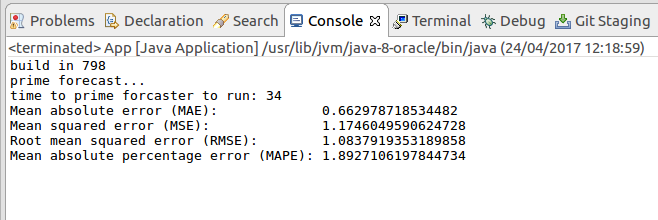
\includegraphics[width=10cm]{img/resultadosSerieDeTiempo1.png}
	\label{fig:resultadosMetricasSerieTiempo}
%\end{SCfigure}
\end{wrapfigure}
Los datos en rojo que aparecen de el 13 al 14 de mayo, son los datos pronosticados por el modelo, y los datos en azul del 13 al 14 de mayo son los datos de pruebas, es decir, lo que en realidad pasó en ese periodo y se usaron para calcular el error, lo resultados de las métricas de error aparecen en la \hyperref[fig:resultadosMetricasSerieTiempo]{figura \ref{fig:resultadosMetricasSerieTiempo}}.

\begin{figure}[!b]
	\centering
	%imagen sin escalar
	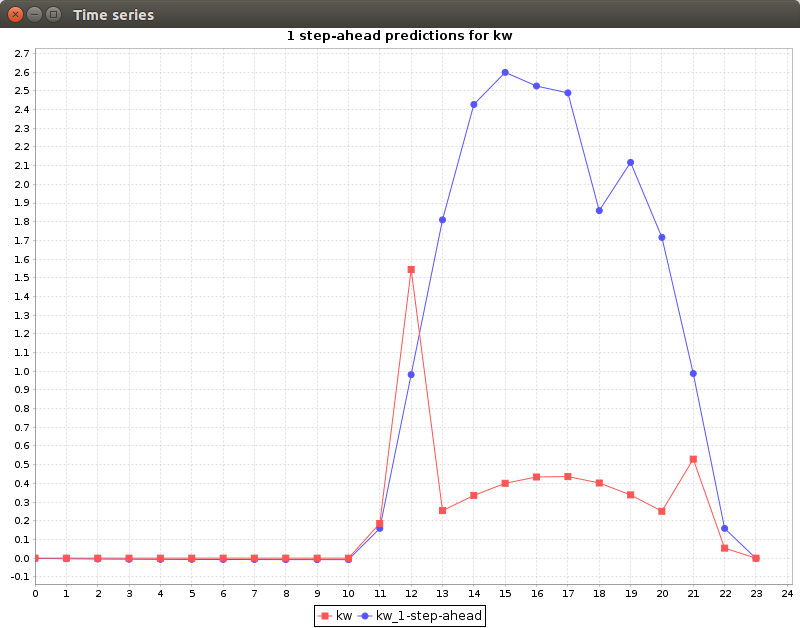
\includegraphics[width=13cm]{img/JFreeChartDriver.png}
	\caption{Ventana generada con la clase JFreeChartDriver. }
	\label{fig:JFreeChartDriver}
\end{figure}
\begin{figure}[!h]
	\centering
	%imagen sin escalar
	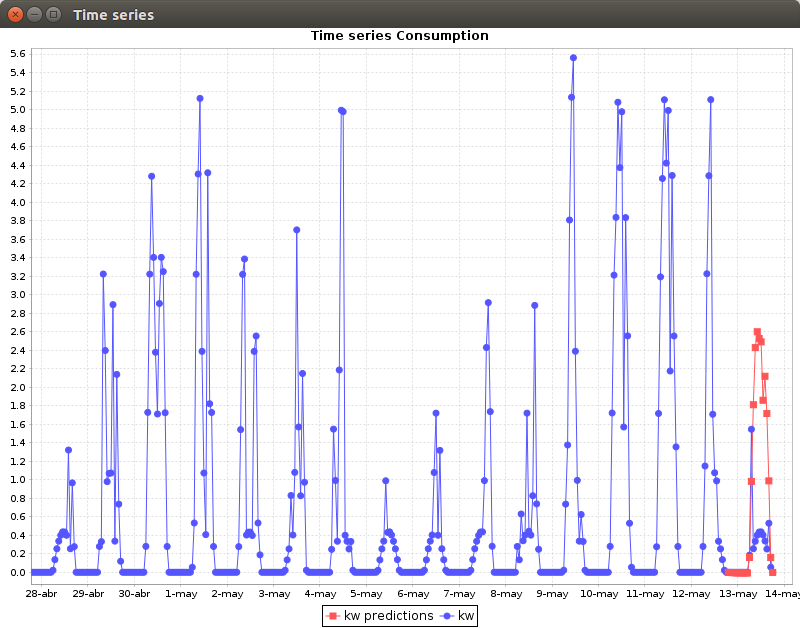
\includegraphics[width=13cm]{img/UtilgraphSeries.png}
	\caption{Ventana generada por el método personalizado Util.graphSeries.}
	\label{fig:Util.graphSeries}
\end{figure}

\subsection{Implementación de redes bayesianas} \label{subsec:implementacionRedes}
\subsubsection{Filtrado}
\label{sec:filtrado}
Ya que las redes bayesianas solo pueden tratar con probabilidades de datos dizcretos, como se vio en la 
\hyperref[subsec:redesbayesianas]{ sección \ref{subsec:redesbayesianas}} de la pagina \pageref{subsec:redesbayesianas}, se necesita aplicar un filtro a los datos que discretize los campos numéricos para que la red bayesiana pueda crear un modelo de los datos, así que se programaron una serie de funciones con este propósito. Se hizo el método \texttt{discretizeData} en la clase \texttt{BayesianNetwork} que a su vez hizo uso del método \texttt{numericToNominal} para discretizar cada uno de los campos del data set, este método se ve en el  \hyperref[lst:numericToNominal]{código \ref{lst:numericToNominal}}.
La función recibe el conjunto de datos, el indice del atributo a discretizar y el número de posibles valores para la variable discreta (en cuantos partes iguales dividir el intervalo entre el valor mínimo y el máximo de la variable).
Lo que hace esta función primero es encontrar el valor mínimo y el máximo en la variable (líneas 101-106), después calcular de que tamaño van a ser cada uno de los rangos que van a representar las variables discretas, y con esto después crea las etiquetas de los rangos (en el for de la línea 114-130) y después dizcretiza los valores de las variables eligiendo un rango en la que el valor de cada variable cae (línea 134-144).
Así que los datos de la \hyperref[fig:datos]{figura \ref{fig:datos}} de la pagina \pageref{fig:datos} después de discretizarse se convierte en los datos de la \hyperref[fig:datosDiscretizados]{figura \ref{fig:datosDiscretizados}}. 

\lstset{language=Java, label=lst:numericToNominal, caption={[Método \texttt{numericToNominal} de la clase \texttt{BayesianNetwork}] Método \texttt{numericToNominal} de la clase \texttt{BayesianNetwork}},
tabsize=3 ,numbers=left,  stepnumber=1, firstnumber=100}

\begin{lstlisting}[frame=single]  
Instances numericToNominal(Instances data, int att, int n){
	double maxi=Double.NEGATIVE_INFINITY, mini= Double.MAX_VALUE;
	for (int i = 0; i < data.numInstances(); i++) {
		Instance act=data.get(i);
		maxi= Math.max(act.value(att), maxi);
		mini= Math.min(act.value(att), mini);
	}
	double separacion = (maxi - mini)/ n;
	labelValues = new double[n+1];
	if(debug)
		System.out.println("min "+mini+", max "+maxi+" separacion "
			+separacion);
	labelData.put(att, new LabelData(mini, separacion, n));
	ArrayList<Attribute> arr= new ArrayList<>(data.numAttributes());
	for (int i = 0; i < data.numAttributes(); i++) {
		if(i==att){
			ArrayList<String> labels = new ArrayList<>(n+1);
			for (int j = 0; j < n; j++) {
				labels.add("["+(mini + separacion*(j))+"-" 
					+ (mini + separacion*(j+1)) +")");
				labelValues[j]= mini + separacion*(j+0.5);
			}
			labelValues[n] = mini + separacion*(n+0.5);
			labels.add("["+maxi +"-inf)");
			if(debug)
				System.out.println("labels: " +labels);
			arr.add(new Attribute(data.attribute(att).name(),labels));
		} else{
			arr.add(data.attribute(i));
		}
	}
	Instances newInst= new Instances(data.relationName(),arr,
		data.numInstances());
	newInst.setClassIndex(data.classIndex());
	for (int c = 0; c < data.numInstances(); c++) {
		Instance act=data.get(c);
		double values[] =  new double[data.numAttributes()];
		for (int i = 0; i < data.numAttributes(); i++) {
			if(i==att){
				values[i]= ((act.value(i) - mini) /separacion);
				values[i]= Math.min(n, values[i]);
			} else{
				values[i]= act.value(i);
			}
		}
		newInst.add(Util.instance(values, newInst));
	}
	return newInst;
}
\end{lstlisting}

\begin{figure}[!t]
	\centering
	%imagen sin escalar
	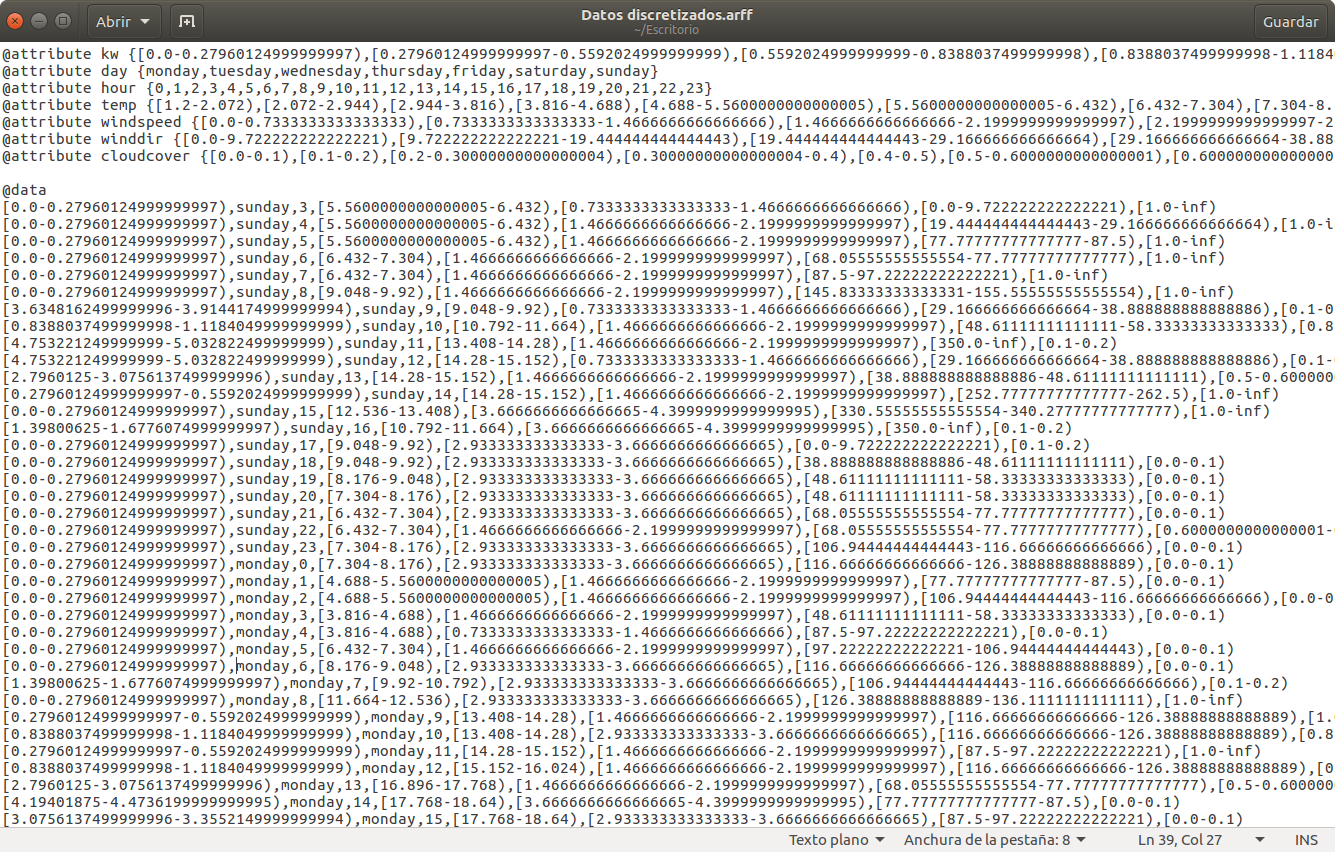
\includegraphics[width=17cm]{img/datosDiscretizados.png}
	\caption{Conjunto de datos después de haber sido discretizados.}
	\label{fig:datosDiscretizados}
\end{figure}

Se puede observar que en la declaración de campos numéricos ahora son de tipo nominal, y los distintos valores que pueden tomar (están entre \{\} después de la declaración del atributo) son etiquetas que representan rangos numéricos con el formato [A-B), donde A y B son variables numéricas de tipo doble.\\
Los datos ahora no aparecen como un número, sino como un rango, y esto permite a la red bayesiana construir el modelo, el cual sera usado para calcular la probabilidad de que una variable caiga en un rango determinado, y esto sera usado para calcular el valor esperado.

\subsubsection{Aplicación del algoritmo}
Al tener el cálculo de las posibilidades de que eventos ocurran se calcula el valor esperado
usando los datos de la distribución de probabilidades calculada por la red bayesiana, por ejemplo, para el caso de que se tenga la  variable que representa los kilowatts producidos en una planta eólica $KW$ , la cual fue discretizada en $n=3$ rangos: 
$KW= \{[0-2), [2-4), [4-\infty)\}$, y la distribución de probabilidad es: 
$DP= \{0.2,~0.5,~0.3\} $; lo cual significa que la probabilidad de que la planta produzca entre 0 y 2 kilowatts es de 0.2, la probabilidad de que se produzca de 2 a 4 kilowatts es de 0.5 y la probabilidad de que se produzca mas de 6 kilowatts es de 0.3. 
Usando estas probabilidades se calcula el valor esperado $\mathbb{E}(KW)$ con la siguiente formula: 
\begin{equation}  \label{eq:valorEsperado}
	\mathbb{E}(KW) = \sum_{i=0}^{n}{LB}_i \cdot {DP}_i 
\end{equation}
Donde $LB$ son las etiquetas de clase de la variable $KW$, es decir un valor que representa al rango, en este caso seria 
$LB=\{1, 3, 6\}$. 
Por lo cual el resultado del valor esperado para este ejemplo seria: $1*0.2 + 3*0.5 + 6*0.3= 3.5$.
En el \hyperref[lst:testAndTrainBayes]{ código \ref{lst:testAndTrainBayes}} se muestra la implementación de este algoritmo desde el filtrado de los datos discutido en la sección de filtrado en pagina \pageref{sec:filtrado} hasta el calculo del valor esperado, y evaluación del modelo para calcular sus métricas de error.

La función que se manda a llamar desde el \texttt{main} es \texttt{trainAndTest}, esta lo primero que hace es aplicarle el filtro de discretización a los datos, con las funciones discutidas en la sección de \hyperref[sec:filtrado]{ filtrado \ref{sec:filtrado}} de la pagina \pageref{sec:filtrado}, y después de esto manda los datos filtrados a la función \texttt{trainAndTestFiltered} en la línea 107, en esta función se manda a construir el modelo con la función \texttt{buildClassifierFiltered} (línea 112), esta función se encuentra implementada en las líneas 133 a la 143, y lo que hace es inicializar los algoritmos de estimación de probabilidades (\texttt{estimator}) y de construcción de la estructura (\texttt{search}) si no hay sido inicializados desde el exterior, y después de esto manda a llamar el método buildClassifier de la clase \texttt{BayesNet}, que es la clase de la librería weka que construye el modelo.\\
Después de construir el modelo, se selecciona el campo o variable a pronosticar, que en este caso se elige la variable de clase (líneas 114-119) por lo que se debe de asignar desde afuera antes de llamar a la función \texttt{trainAndTest} y justo empieza el proceso de pronóstico en el for de la línea 120 a la 128, este for recorre los datos \texttt{test}, que son los que siguen en la línea de tiempo después de los datos \texttt{train} y son los valore reales de lo que ocurrió, para cada uno de estos se hace una predicción (línea 121) usando la función \texttt{classifyInstanceFiltered}, la cual esta implementada en las líneas 144-152 e implementan la ecuación \ref{eq:valorEsperado}. Luego en las líneas 123 a 127 se guardan los valores y se calcula el error con el valor predicho y el valor real (línea 127), esta función lo que hace es sacar la sumatoria y esta implementada en las líneas 153-160, a su vez esta sobre cargada para recibir un entero y terminar el calculo de error, esta función se manda a llamar justo después del for en la línea 129 y esta implementada en las líneas 161 a la 166.

Este código se ejecuta en un \texttt{main} parecido al del \hyperref[lst:maincustomtest]{ código \ref{lst:maincustomtest}}, así que podemos comparar los datos pronosticados con los datos reales de manera gráfica. En la  \hyperref[fig:redBayesianaRes]{ figura \ref{fig:redBayesianaRes}} podemos ver una ventana con los resultados del pronostico usando la red bayesiana, y en la \hyperref[fig:redBayesianaResZoom]{ figura \ref{fig:redBayesianaResZoom}} podemos ver un acercamiento a los datos pronosticados.

\lstset{language=Java, label=lst:testAndTrainBayes, caption={[Métodos para entrenar y evaluar una red bayesiana (clase \texttt{BayesianNetwork})] Métodos para generar predicciones y evaluar el modelo generado de la clase \texttt{BayesianNetwork}},
tabsize=3 ,numbers=left,  stepnumber=1, firstnumber=100}

\begin{lstlisting}[frame=single]  
public List<ErrorModule> trainAndTest(Instances train,
		Instances test) throws Exception {
	train=discretizeData(train);
	Instances testFiltered= new Instances(test);
	for (int i = 0; i < test.size(); i++) {
		discretize(testFiltered.get(i));
	}
	return trainAndTestFiltered(train, testFiltered, test);
}
public List<ErrorModule> trainAndTestFiltered(Instances train, 
		Instances testFiltered, Instances test) throws Exception {
	List<ErrorModule> preds= new ArrayList<>(1);
	buildClassifierFiltered(train);

	String fieldsToForecast= train.classAttribute().name();
	ErrorModule em= new ErrorModule();
	List<String> f=new ArrayList<String>();
	f.add(fieldsToForecast);
	em.setTargetFields(f);
	Attribute att= testFiltered.attribute(fieldsToForecast);
	for (int i = 0; i < testFiltered.numInstances(); i++) {			
		double value= classifyInstanceFiltered(testFiltered.get(i));
		List<NumericPrediction> predsForStepI = new ArrayList<>(1);
		NumericPrediction pred= 
			new NumericPrediction(test.get(i).value(att), value);
		predsForStepI.add(pred);
		em.evaluateForInstance(predsForStepI, test.get(i));
		calculateErrors(pred.actual(), pred.predicted());
	}
	calculateErrors(testFiltered.numInstances());
	preds.add(em);
	return preds;
}
protected void buildClassifierFiltered(Instances filteredData)
		throws Exception{
	if(estimator==null)
		estimator=new SimpleEstimator();
	if(search==null)
		search=new K2();
	this.data = filteredData; 
	red.setEstimator(estimator);
	red.setSearchAlgorithm(search);
	red.buildClassifier(filteredData);
}
protected double classifyInstanceFiltered(Instance instance) 
		throws Exception{
	double distr[]=red.distributionForInstance(instance);
	double r=0;
	for (int i = 0; i < distr.length; i++) {
		r+= labelValues[i]*distr[i];
	}
	return r;
}
protected void calculateErrors(double actual, double predicted) {
	double diff= predicted- actual;
	MAE+= Math.abs(diff);
	MSE+= diff*diff;
	if(actual!=0){
		MAPE+= Math.abs(diff /actual);
	}
}
protected void calculateErrors(int n){
	MAE= MAE/n;
	MSE= MSE/n;
	RMSE= Math.sqrt(MSE);
	MAPE=MAPE/n;
}
\end{lstlisting}

\begin{figure}[!h]
	\centering
	%imagen sin escalar
	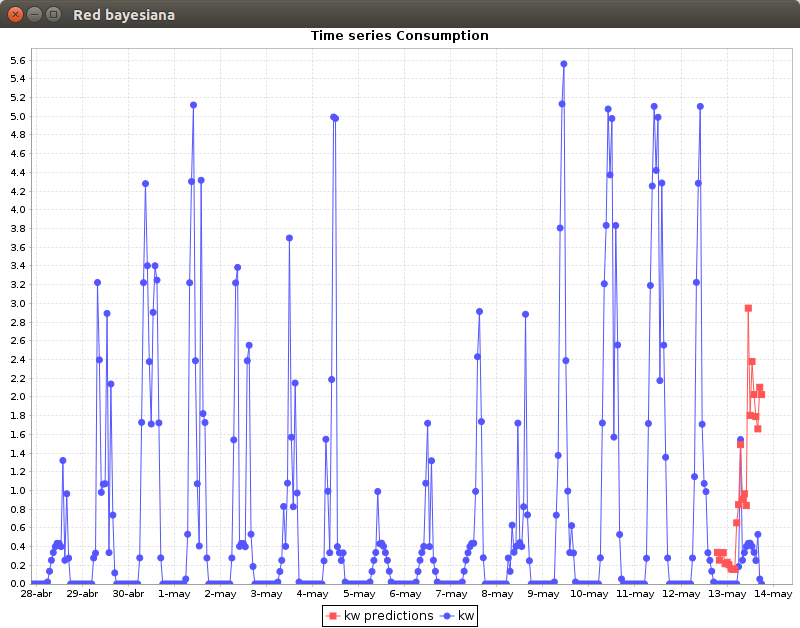
\includegraphics[width=13.5cm]{img/redBayesianaRes.png}
	\caption{Gráfica de resultados de pronostico de red bayesiana.}
	\label{fig:redBayesianaRes}
\end{figure}

\begin{figure}[ht]
	\centering
	%imagen sin escalar
	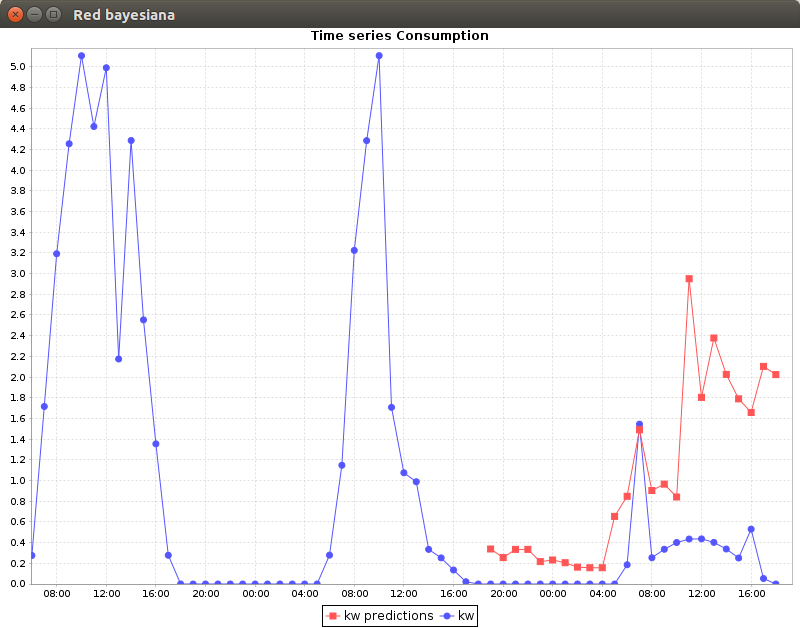
\includegraphics[width=13.5cm]{img/redBayesianaResZoom.png}
	\caption{Acercamiento a conjunto de datos después de haber sido discretizados.}
	\label{fig:redBayesianaResZoom}
\end{figure}

\section{Comparación de algoritmos} \label{sec:comparacion}
Una de las principales diferencias entre una red bayesiana con una la serie de tiempo es que el pronóstico con red bayesiana requiere datos sobre el futuro (los otros datos que no son la variable a predecir), es decir los datos del clima. Otros campos como los de hora y día de la semana si se conocen al momento de querer predecir una fecha y hora, pues si se sabe que fecha y hora se quieren predecir, se puede saber que día de la semana y que hora sera.
Las pruebas que se hicieron aquí fueron con los datos reales, es decir se ocuparon los datos del clima como si ya supiéramos como estará el clima, pero en la realidad lo que se usara para implementar la solución en el broker, serán los datos del reporte del clima dado por el servidor.

\subsection{Series de tiempo} \label{subsec:compSeries}
Recordando el funcionamiento interno del la implementación de series de tiempo de la libreria weka, esta transforma el modelo agregándole variables de arrastre, y después aprende el modelo con un algoritmo base, el algoritmo que se uso en las demostraciones pasadas fue el de regresión lineal, implementado en la clase 
\texttt{weka.classifiers.functions.LinearRegression}, lo siguiente que se hizo fue probar cual de los algoritmos posibles es el que da mejores resultados, así que se comenzó por hacer un arreglo llamado \texttt{baseLearners} en la clase \texttt{TimeSeries}, el cual se inicializo con la función \texttt{TimeSeries.createSearchAlgorithms()} la cual aparece en el 
\hyperref[lst:createSearchAlgorithms]{ código \ref{lst:createSearchAlgorithms}}, aquí podemos ver todos los algoritmos que podemos usar para aprender el modelo de series de tiempo. %este parrafo es renderizado diferente aqui que en la lap, aqui ocupa una linea menos

\lstset{language=Java, label=lst:createSearchAlgorithms, caption={[Método \texttt{createSearchAlgorithms} de la clase \texttt{TimeSeries}] Método \texttt{createSearchAlgorithms} de la clase \texttt{TimeSeries}},
tabsize=3 ,numbers=left,  stepnumber=1, firstnumber=100}

\begin{lstlisting}[frame=single]  
public void createSearchAlgorithms(){
	LinearRegression  lr= new LinearRegression();
	MultilayerPerceptron ml= new MultilayerPerceptron();
	IBk ib= new IBk();
	KStar ks= new KStar();
	LWL lw= new LWL();
	AdditiveRegression adr= new AdditiveRegression();
	Bagging ba= new Bagging();
	CVParameterSelection cv= new CVParameterSelection();
	MultiScheme ms= new MultiScheme();
	RandomCommittee rc= new RandomCommittee();
	RandomizableFilteredClassifier rf= 
		new RandomizableFilteredClassifier();
	RandomSubSpace rs= new RandomSubSpace();
	DecisionTable dt= new DecisionTable();
	M5Rules m5= new M5Rules();
	ZeroR zr= new ZeroR();
	DecisionStump ds= new DecisionStump(); //trees
	M5P m5p= new M5P();
	RandomForest rft=new RandomForest();
	RandomTree rt= new RandomTree();
	REPTree rpt= new REPTree();
	baseLearners= new Classifier[]{lr, ml, ib, ks, lw, adr,
		ba, cv, ms, rc, rf, rs, dt, m5, zr, ds, m5p, rft, rt, rpt};
}
\end{lstlisting}

Todos los algoritmos guardados en el arreglo \texttt{baseLearners} de la clase \texttt{TimeSeries} en el \hyperref[lst:createSearchAlgorithms]{ código \ref{lst:createSearchAlgorithms}}, se usan en el método \texttt{findBestConfigTimeSeries}, que aparece en el 
\hyperref[lst:findBestConfigTimeSeries]{ código \ref{lst:findBestConfigTimeSeries}} el cual construyen el modelo con cada uno de los algoritmos guardados en este arreglo, y compara los resultados de acuerdo a su error medio absoluto (MAE), imprimiendo al final el resultado de que algoritmo tuvo mejor desempeño, y una gráfica con los datos de pronostico del mejor algoritmo.
Se puede observar que el 
\hyperref[lst:findBestConfigTimeSeries]{ código \ref{lst:findBestConfigTimeSeries}} tiene líneas en común con 
el \hyperref[lst:maincustomtest]{ código \ref{lst:maincustomtest}}, en especifico de la línea 102 a la 127, ya que estas lineas se encargan de cargar los datos (102-104), especificar los campos objetivo (a pronosticar) y de tiempo (105-106), dividir el los datos en un dataset de entrenamiento y uno para pruebas (108-111), especificar la periodicidad (112-119), y crear el objeto \texttt{timeseries} que encapsula el analisis de la serie de tiempo (121-127).

\lstset{language=Java, label=lst:findBestConfigTimeSeries, caption={[Método \texttt{findBestConfigTimeSeries}] Método \texttt{findBestConfigTimeSeries}},
tabsize=3 ,numbers=left,  stepnumber=1, firstnumber=100}

\begin{lstlisting}[frame=single]  
public static void findBestConfigTimeSeries(){
try { 
	Instances datos =
		Util.instancesFromFile("SOLAR_PRODUCTION.arff");

	String targetName="kw" ;
	String xaxis="date";
	
	int numInstPred=24;
	int size=datos.numInstances();
	Instances train=new Instances(datos, 0, size - numInstPred);
	Instances test=new Instances(datos,size-numInstPred,numInstPred);
	String periodicTest=
		"day=>=*:*:*:*:*:*:*:6:*:* <=*:*:*:*:*:*:*:18:*:*";
	
	NewLagMaker lag=new NewLagMaker();
	lag.setIncludePowersOfTime(false);
	lag.setIncludeTimeLagProducts(false);
	lag.setPrimaryPeriodicFieldName("hour"); 
	lag.addCustomPeriodic(periodicTest);
	
	TimeSeries timeseries = new TimeSeries();
	timeseries.setDebug(true);
	timeseries.setTimestamp(xaxis);
	timeseries.setFieldsToForecast(targetName);
	timeseries.forecaster.setTSLagMaker(lag);
	timeseries.setHorizon(24);
	timeseries.setPrimeWindowSize(24);
	timeseries.createSearchAlgorithms();
	double mae= Double.MAX_VALUE;
	int bestBase=0;
	List<ErrorModule> preds, best=null;
	long time;

	for (int i = 0; i < timeseries.baseLearners.length; i++) {
		timeseries.reset();
		timeseries.setBaseLearner(timeseries.baseLearners[i]);
		time= System.currentTimeMillis();
		preds= timeseries.test(train, test);
		if(timeseries.getMAE() <mae){
			mae= timeseries.getMAE();
			bestBase=i;
			best= preds;
		}
		System.out.printf("%s\nMAE: %4.7f MSE: %4.7f RMSE: %4.7f MAPE: "
			+"%4.7f time %d \n", timeseries.baseLearners[i].getClass()
			.getName(),timeseries.getMAE(),timeseries.getMSE(),timeseries
			.getRMSE(),timeseries.getMAPE(),System.currentTimeMillis()
			- time);
	}
	System.out.println("Best:\n"
		+timeseries.baseLearners[bestBase].getClass().getName());
	System.out.print("MAE: "+ mae);
	JPanel graph=Util.graphSeries(best.get(0),datos,targetName,xaxis);
	JFrame jf = new JFrame("Serie de tiempo " 
		+timeseries.baseLearners[bestBase].getClass().getName());
	jf.setDefaultCloseOperation(JFrame.DISPOSE_ON_CLOSE);
	jf.setSize(800, 600);
	jf.getContentPane().setLayout(new BorderLayout());
	jf.getContentPane().add(graph, BorderLayout.CENTER);
	jf.setVisible(true);
} catch (Exception e) {
	e.printStackTrace();
}
}
\end{lstlisting}

En el for de la linea 134 se realiza la comparación de los algoritmos, primero reinicia el objeto \texttt{timeseries} en la linea 135 y en la 136 
le asigna un algoritmo encapsulado en uno de los objetos del arreglo \texttt{TimeSeries.baseLearners} de la
clase \texttt{Classifier}
del \hyperref[lst:createSearchAlgorithms]{ código \ref{lst:createSearchAlgorithms}}. La linea 137 solo sirve para poder calcular cuanto se tardo la evaluación del algoritmo (construir el modelo, extrapolar los datos y comparar los resultados con los reales) en la linea 138. El if de la linea 139-143 se encarga de guardar el mejor algoritmo y sus resultados y en la linea 144 se imprimen los resultados de la evaluación del algoritmo \texttt{i}.
Por ultimo después del for (150-160) se imprimen los resultados del mejor algoritmo y se grafican los datos en una ventana. 
En la \hyperref[fig:resultadosCompSeries]{figura \ref{fig:resultadosCompSeries}} se muestra la consola con los últimos resultados de la ejecución del \hyperref[lst:findBestConfigTimeSeries]{ código \ref{lst:findBestConfigTimeSeries}}

\begin{figure}[ht]
	\centering
	%imagen sin escalar
	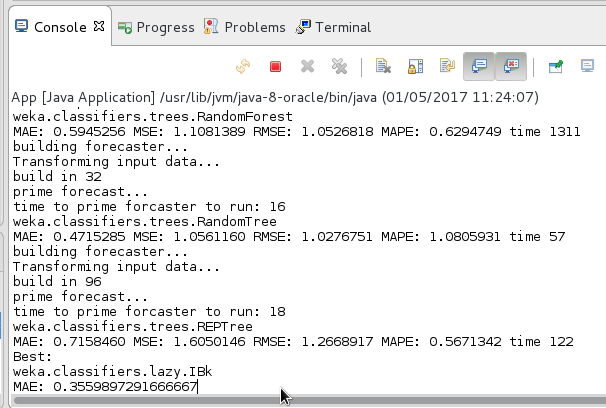
\includegraphics[width=15cm]{img/resultadosComparacionSeries.png}
	\caption{Resultados de la comparación de los algoritmos de series de tiempo.}
	\label{fig:resultadosCompSeries}
\end{figure}
El programa imprimió para cada uno de los algoritmos ejecutados, información del progreso (\texttt{building forecaster...,Transforming input data..., build in 96}, etc), el nombre de la clase que encapsula el algoritmo (\texttt{weka.classifiers.trees.REPTree}), métricas de error: error medio absoluto (MAE), error medio cuadrado (MSE), raiz de error medio cuadrado (RMSE) y error porcentual medio absoluto (MAPE), y el tiempo que tardo en ejecutar la prueba. Al final se imprimió la clase con el algoritmo que tuvo el mejor desempeño y su error medio absoluto, la cual fue en este caso \texttt{weka.classifiers.lazy.IBk}.
En la \hyperref[fig:graficaResultadosCompSeries]{figura \ref{fig:graficaResultadosCompSeries}} se muestra la ventana con la gráfica de los datos del mejor algoritmo. En esta prueba se hizo una predicción a 48 horas.

\begin{figure}[ht]
	\centering
	%imagen sin escalar
	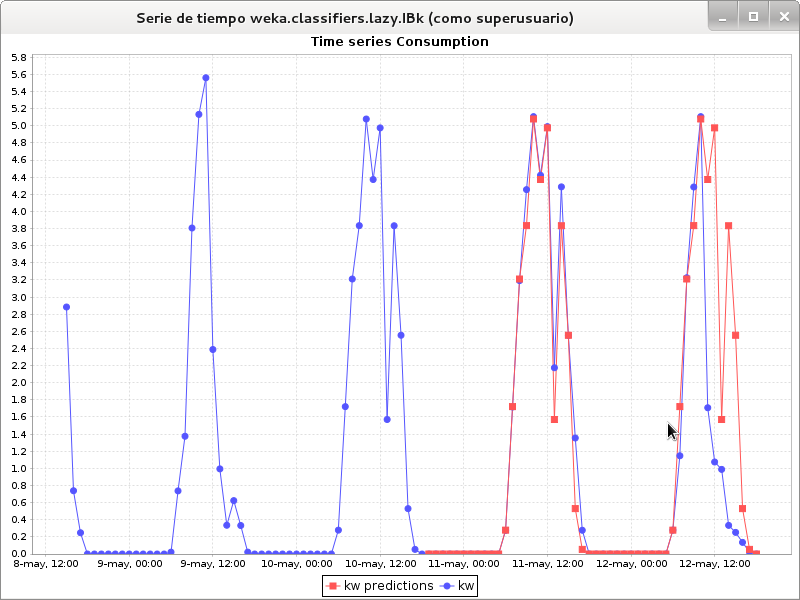
\includegraphics[width=15cm]{img/graficaResultadosCompSeries.png}
	\caption{Gráfica de los resultados de la comparación de los algoritmos de series de tiempo.}
	\label{fig:graficaResultadosCompSeries}
\end{figure}

\subsection{Redes bayesianas} \label{subsec:compRedes}
En el caso de las redes bayesianas, estas necesitan dos algoritmos base para construirse, un algoritmo que aprenda la estructura de la red, y otro que aprenda las probabilidades dentro de la estructura. Al probar los algoritmos para aprender las probabilidades surgieron errores, el estimador \texttt{BMAEstimator} no puede manejar redes con nodos con mas de un padre, y la clase \texttt{MultiNomialBMAEstimator} solo puede soportar atributos nominales binarios, así que el estimador que se uso fue el \texttt{SimpleEstimator}, aunque se dejo la estructura por si en el futuro se agrega otro algoritmo, eso se creo en el método \texttt{createEstimators} en la clase \texttt{BayesianNetwork}, el cual aparece en el 
\hyperref[lst:createLearners]{código \ref{lst:createLearners}}.
Los algoritmos para aprender la estructura de la red bayesiana se crearon en el método \texttt{createSearchAlgorithms} de la clase \texttt{BayesianNetwork}, el cual aparece en el 
\hyperref[lst:createLearners]{código \ref{lst:createLearners}}, podemos ver que ciertos algoritmos reciben parámetros, estos se declararon al principio del método, los parámetros son: 

\begin{enumerate}
	\item \texttt{markov}: Cuando se le asigna true, después de que la estructura de la red es creada se le
		aplica una corrección de manta de Markov. Esto asegura que todos los nodos en la red son parte de la
		manta de Markov del nodo objetivo (la variable que se desea predecir).
	\item \texttt{initAsNaive}: Cuando se le asigna true, la red inicial usada es una Naive Bayes (red ingenua de Bayes), la cual es una red con una flecha desde el nodo objetivo a todos los demás nodos.
	\item \texttt{maxNumPar}: El numero máximo de padres que un nodo en la red puede tener.
	\item \texttt{scoretype}: Determina el tipo de medición usada para juzgar la calidad de una estructura de
			red, esta puede ser uno de los valores: Bayes, BDeu, Minimum Description Length (MDL), Akaike 
			Information Criterion (AIC), y Entropy.
\end{enumerate}

\lstset{language=Java, label=lst:createLearners, caption={[Métodos \texttt{createEstimators} y \texttt{createSearchAlgorithms}] Métodos \texttt{createEstimators} y \texttt{createSearchAlgorithms}},
tabsize=3 ,numbers=left,  stepnumber=1, firstnumber=100}

\begin{lstlisting}[frame=single]  
protected void createEstimators(){
	SimpleEstimator simple= new SimpleEstimator();
	estimators= new BayesNetEstimator[]{ simple/*,bma, mn*/}; 
}
protected void createSearchAlgorithms(){
	boolean markov= false, initAsNaive=false; int maxNumPar= 1;
	SelectedTag scoretype= new SelectedTag(0, 
		LocalScoreSearchAlgorithm.TAGS_SCORE_TYPE);//0-4
	file= "maxNumPar " + maxNumPar+ " initAsNaive " + initAsNaive+ 
		" markov "+ markov+ " scoretype " + scoretype.getSelectedTag()
		.getReadable();
	if(debug)
		System.out.println(file);
	
	GeneticSearch gs= new GeneticSearch();
	gs.setDescendantPopulationSize(100);
	gs.setPopulationSize(10);
	gs.setRuns(10);	
	gs.setMarkovBlanketClassifier(markov);
	gs.setUseCrossOver(true);
	gs.setUseMutation(true);		
	gs.setScoreType(scoretype);
	HillClimber hc=  new HillClimber();
	hc.setInitAsNaiveBayes(initAsNaive);
	hc.setMaxNrOfParents(maxNumPar);
	hc.setUseArcReversal(useArcR);
	hc.setMarkovBlanketClassifier(markov);
	hc.setScoreType(scoretype);
	K2 k2= new K2();
	k2.setInitAsNaiveBayes(initAsNaive);
	k2.setMarkovBlanketClassifier(markov);
	k2.setMaxNrOfParents(maxNumPar);
	k2.setRandomOrder(false);
	k2.setScoreType(scoretype);
	LAGDHillClimber lagd= new LAGDHillClimber();
	lagd.setInitAsNaiveBayes(initAsNaive);
	lagd.setMarkovBlanketClassifier(markov);
	lagd.setMaxNrOfParents(maxNumPar);
	lagd.setNrOfGoodOperations(5);
	lagd.setNrOfLookAheadSteps(2);
	lagd.setScoreType(scoretype);
	lagd.setUseArcReversal(useArcR);
	RepeatedHillClimber rhc= new RepeatedHillClimber();
	rhc.setInitAsNaiveBayes(initAsNaive);
	rhc.setMarkovBlanketClassifier(markov);
	rhc.setMaxNrOfParents(maxNumPar);
	rhc.setRuns(10);
	rhc.setScoreType(scoretype);
	SimulatedAnnealing sa= new SimulatedAnnealing();
	sa.setDelta(0.999);
	sa.setRuns(1000);
	sa.setMarkovBlanketClassifier(markov);
	sa.setTStart(10);
	sa.setScoreType(scoretype);
	TabuSearch tb= new TabuSearch();
	tb.setInitAsNaiveBayes(initAsNaive);
	tb.setMarkovBlanketClassifier(markov);
	tb.setMaxNrOfParents(maxNumPar);
	tb.setRuns(10);
	tb.setScoreType(scoretype);
	tb.setTabuList(5);
	TAN tan= new TAN();
	tan.setMarkovBlanketClassifier(markov);
	tan.setScoreType(scoretype);
	searches= new SearchAlgorithm[]
		{sa, gs, hc,k2, lagd, rhc, tb, tan};
}
\end{lstlisting}

Todos estos algoritmos se ponen a prueba de la misma manera que en el 
\hyperref[lst:findBestConfigTimeSeries]{código \ref{lst:findBestConfigTimeSeries}}, se corren todos uno por uno y se toma al que tiene menor error medio absoluto, la diferencia es que esta vez se ejecuto varias veces, puesto que los algoritmos toman 4 parámetros (\texttt{markov, initAsBayes, maxNumPar, scoretype}), se ejecuto una vez para cada combinación de parámetros, es decir con \texttt{markov} e \texttt{initAsBayes} en true y false, esas son 4 combinaciones, con \texttt{maxNumPar} con valores de 1 a 3, son 3 combinaciones más,y la variable \texttt{scoretype} toma 4 valores posibles, por lo que el total de combinaciones de parámetros y el numero de veces que se ejecuto este método fue de $4*3*4 = 48$. 
Un ejemplo de los resultados de estas pruebas se muestra en la 
\hyperref[fig:resultadosComparacionRed]{figura \ref{fig:resultadosComparacionRed}}, en donde los parámetros son \texttt{maxNumPar=1 initAsNaive=false markov=false scoretype=BAYES}, y el mejor algoritmo en este caso fue el \texttt{HillClimber}. 
La \hyperref[fig:GraficaResultadosCompRed]{ figura \ref{fig:GraficaResultadosCompRed}} muestra una ventana con una gráfica de los resultados de esta comparación. 
Por los resultados de la 
\hyperref[fig:resultadosCompSeries]{ figura \ref{fig:resultadosCompSeries}} y de la
\hyperref[fig:resultadosComparacionRed]{figura \ref{fig:resultadosComparacionRed}}, podemos ver que el algoritmo de series de tiempo tuvo un ligeramente mejor desempeño, ya que su MAE fue de 0.3559, mientras que el de la red bayesiana fue de 0.3872, pero esto depende mucho de la situación, ya que se hicieron varias pruebas con distintos datos y en algunos la red bayesiana daba un mejor desempeño.


\begin{figure}[ht]
	\centering
	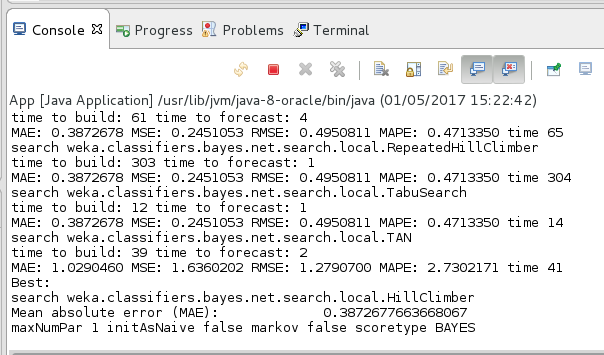
\includegraphics[width=15cm]{img/resultadosComparacionRed.png}
	\caption{Resultados de la comparación de algoritmos de aprendizaje de redes bayesianas.}
	\label{fig:resultadosComparacionRed}
\end{figure}

\begin{figure}[!ht]
	\centering
	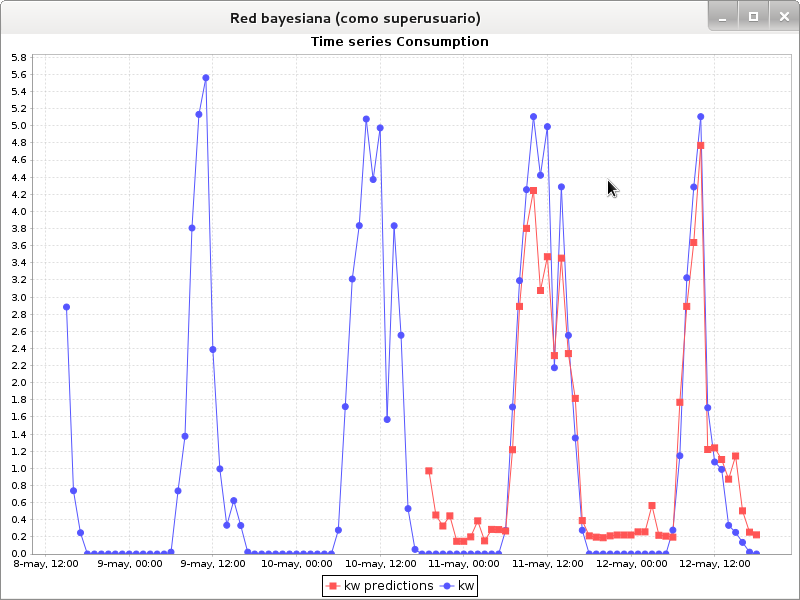
\includegraphics[width=15cm]{img/graficaResultadosCompRed.png}
	\caption{Gráfica del resultado de la comparación algoritmos de aprendizaje de redes bayesianas.}
	\label{fig:GraficaResultadosCompRed}
\end{figure}

Como ejemplo de el caso en que la red bayesiana resulta mejor que la serie de tiempo, está la 
figura \ref{fig:graficaRedBayesianaIrregluar} y \ref{fig:graficaSerieIrregluar}, 
en donde se uso un set de datos en donde un día estaba muy nublado y la producción de energía solar fue menor, esta variable climática si la tomo en cuenta de manera correcta la red bayesiana y la serie de tiempo no, dando como resultado que la red bayesiana fuera mejor con un MAE de 0.3225 usando el algoritmo de aprendizaje \texttt{weka.classifiers.bayes.net.search.local.K2} con los parámetros \texttt{maxNumPar=1 initAsNaive=false markov=false scoretype=BDeu}, en cambio la serie de tiempo tuvo un menor desempeño teniendo un error MAE mayor de 0.4437 usando el algoritmo de aprendizaje \texttt{weka.classifiers.trees.RandomForest}.

\begin{figure}[!h]
	\centering
	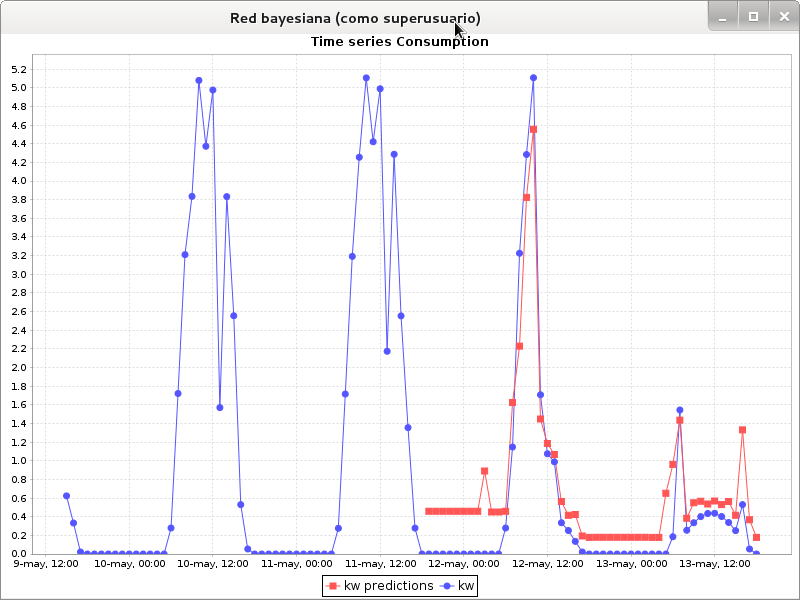
\includegraphics[width=11cm]{img/graficaRedBayesianaIrregluar.png}
	\caption{Gráfica del pronostico de una red bayesiana en un ambiente irregular.}
	\label{fig:graficaRedBayesianaIrregluar}
\end{figure}

\begin{figure}[!h]
	\centering
	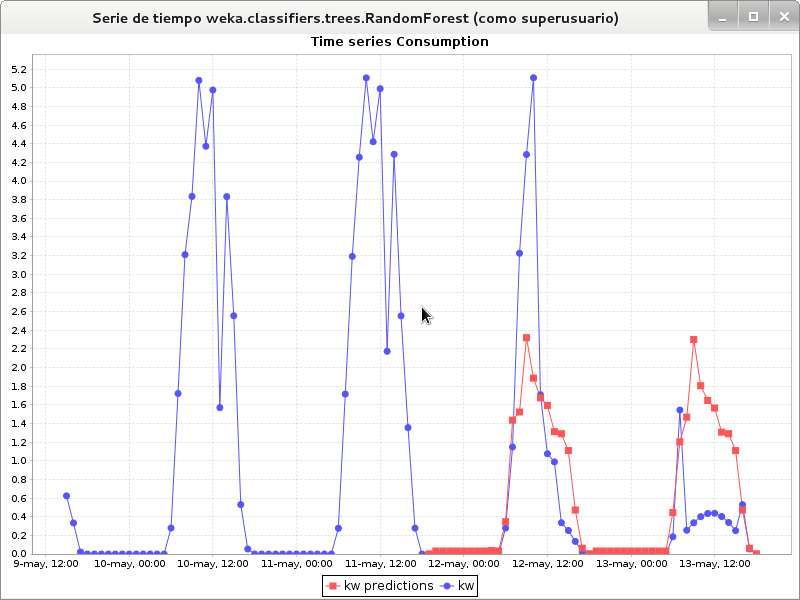
\includegraphics[width=11cm]{img/graficaSerieIrregluar.png}
	\caption{Gráfica del pronostico de una serie de tiempo en un ambiente irregular.}
	\label{fig:graficaSerieIrregluar}
\end{figure}

Con las comparaciones hechas en el algoritmo de series de tiempo se puede concluir que lo que hace es encontrar cierto patrón de repetición, y cuando se le pide que pronostique a futuro, lo que hace es repetir este patrón, tal como se ve en la figuras 
\ref{fig:graficaResultadosCompSeries} y \ref{fig:graficaSerieIrregluar}, en donde repitió el patrón casi exactamente igual; en la 
\hyperref[fig:graficaResultadosCompSeries]{ figura \ref{fig:graficaResultadosCompSeries}} se observa que acertó la predicción del primer día, pero la del segundo fue mas errado. En la 
\hyperref[fig:graficaSerieIrregluar]{ figura \ref{fig:graficaSerieIrregluar}} hizo un pronostico pobre desde el principio, y solamente lo repitió para el primero y segundo día.\\
El algoritmo de redes bayesianas puede tomar en cuenta las variables del clima, lo cual le permite hacer predicciones mas acertadas cuando el clima es un factor importante, cuando el clima no es un factor importante el algoritmo de series de tiempo tiene un desempeño parecido a la de la red bayesiana, así que en conclusión el uso de un algoritmo o de otro depende de la situación que se tenga y de la procedencia de los datos, por ejemplo, las plantas solares y eólicas dependen mucho del clima, por lo que el uso de una red bayesiana es mas apropiado para la predicción de la producción de estas, mientras que para otro tipo de clientes puede ser suficiente una serie de tiempo.

